\chapter{Basic OWL}
\label{ch12}

In previous chapters, we saw how RDFS-Plus as a modeling system provides
considerable support for distributed information and federation of
information. Simple constructs in RDFS-Plus can be combined in various
ways to match properties, classes, and individuals. In the previous
chapter, we saw this utility applied to knowledge organization (SKOS).
In this chapter, we present the modeling capabilities of OWL that go
beyond RDFS-Plus.

The OWL Recommendation is now in version 2.0, which extends the
capabilities of OWL 1.0 with a number of new modeling constructs, but
does not change the fundamental principles of how OWL works. Most of the
modeling patterns in this book are valid in both OWL 1.0 as well as OWL
2.0; when something is specifically only available in OWL 2.0, we will
indicate it explicitly.

We begin our presentation of OWL with a treatment of owl:Restriction.
This single
construct enhances the representational power of OWL by allowing us to
describe classes in terms of other things we have already modeled. As we
shall see, this opens up whole new vistas in modeling capabilities.

\section{Restrictions}

Suppose we have defined in RDFS a class we call \texttt{BaseballTeam}, with a
particular subclass called \texttt{MajorLeagueTeam}, and another class we call
\texttt{BaseballPlayer}. The roster for any particular season would be
represented as a property \texttt{playsFor} that relates a \texttt{BaseballPlayer} to a
\texttt{BaseballTeam}. Certain players are special in that they play for a
\texttt{MajorLeagueTeam}. We'd like to define that class and call it
\texttt{MajorLeaguePlayer} (or  "Major League Players"  when we're talking about them in the text). If we are interested in the fiscal side of baseball, we
could also be
interested in the class of Agents who represent Major League Players,
and then the bank accounts controlled by the Agents who represent Major
League Players and so on.

One of the great powers of the Semantic Web is that information that has
been specified by one person in one context can be reused either by that
person or by others in different contexts. There is no expectation that
the same source who defined the roster of players will be the one that
defines the role of the agents or of the bank accounts. If we want to
use information from multiple sources together, we need a way to express
concepts from one context in terms of concepts from the other. In OWL,
this is achieved by having a facility with which we can describe new
classes in terms of classes that have already been defined. This
facility can also be used to model more complex constructs than the ones
we've discussed so far.

We have already seen how to define simple classes and relationships
between them in RDFS and RDFS-Plus (which is a subset of OWL), but none of the constructs we have seen so
far can create descriptions of the sort we want in our Major League
Baseball Player example. This is done in OWL using a language construct
called a \texttt{Restriction}.

Consider the case of a \texttt{MajorLeaguePlayer}. We informally defined a \texttt{MajorLeaguePlayer} as someone who plays on a \texttt{MajorLeagueTeam}. The intuition
behind the name \texttt{Restriction} is that membership in the class
\texttt{MajorLeaguePlayer} is \emph{restricted} to those things that play for a
\texttt{MajorLeagueTeam}. Since a \texttt{Restriction} is a special case of a \texttt{Class}, we
will sometimes refer to a \texttt{Restriction} as a \emph{Restriction Class} just to
make that point clear.

More generally, a \texttt{Restriction} in OWL is a \texttt{Class} defined by describing
the individuals it contains. This simple idea forms the basis for
extension of models in OWL: If you can describe a set of individuals in
terms of known classes, then you can use that description to define a
new class. Since this new class is now also an existing class, it can be
used to describe individuals for inclusion in a new class, and so on. We
will return to the baseball player example later in this chapter, but
first we need to learn more about the use of restriction classes.

\begin{example}{Questions and Answers}
\label{ex:ch12.1}

To start with, we will use a running example of managing questions and
answers, as if we were modeling a quiz, examination, or questionnaire.
This is a fairly simple area that nevertheless illustrates a wide
variety of uses of restriction classes in OWL.

Informally, a questionnaire consists of a number of questions, each of
which has a number of possible
answers. A question includes string data for the text of the question,
whereas an answer includes string data for the text of the answer. In
contrast to a quiz or examination, there are typically no ``right''
answers in a questionnaire. In questionnaires, quizzes, and
examinations, the selection of certain answers may preclude the posing
of other questions.

This basic structure for questionnaires can be represented by classes
and properties in OWL. Any
particular questionnaire is then represented by a set of individual
questions, answers, and concepts and particular relationships between
them.

The basic schema for the questionnaire is as follows and is shown
diagrammatically in Figure~\ref{fig:ch12.01}.

Throughout the example, we will use the namespace \texttt{q:} to refer to
elements that relate to questionnaires in general, and the namespace \texttt{d:}
to refer to the elements of the particular example questionnaire.

\begin{figure}
\centering
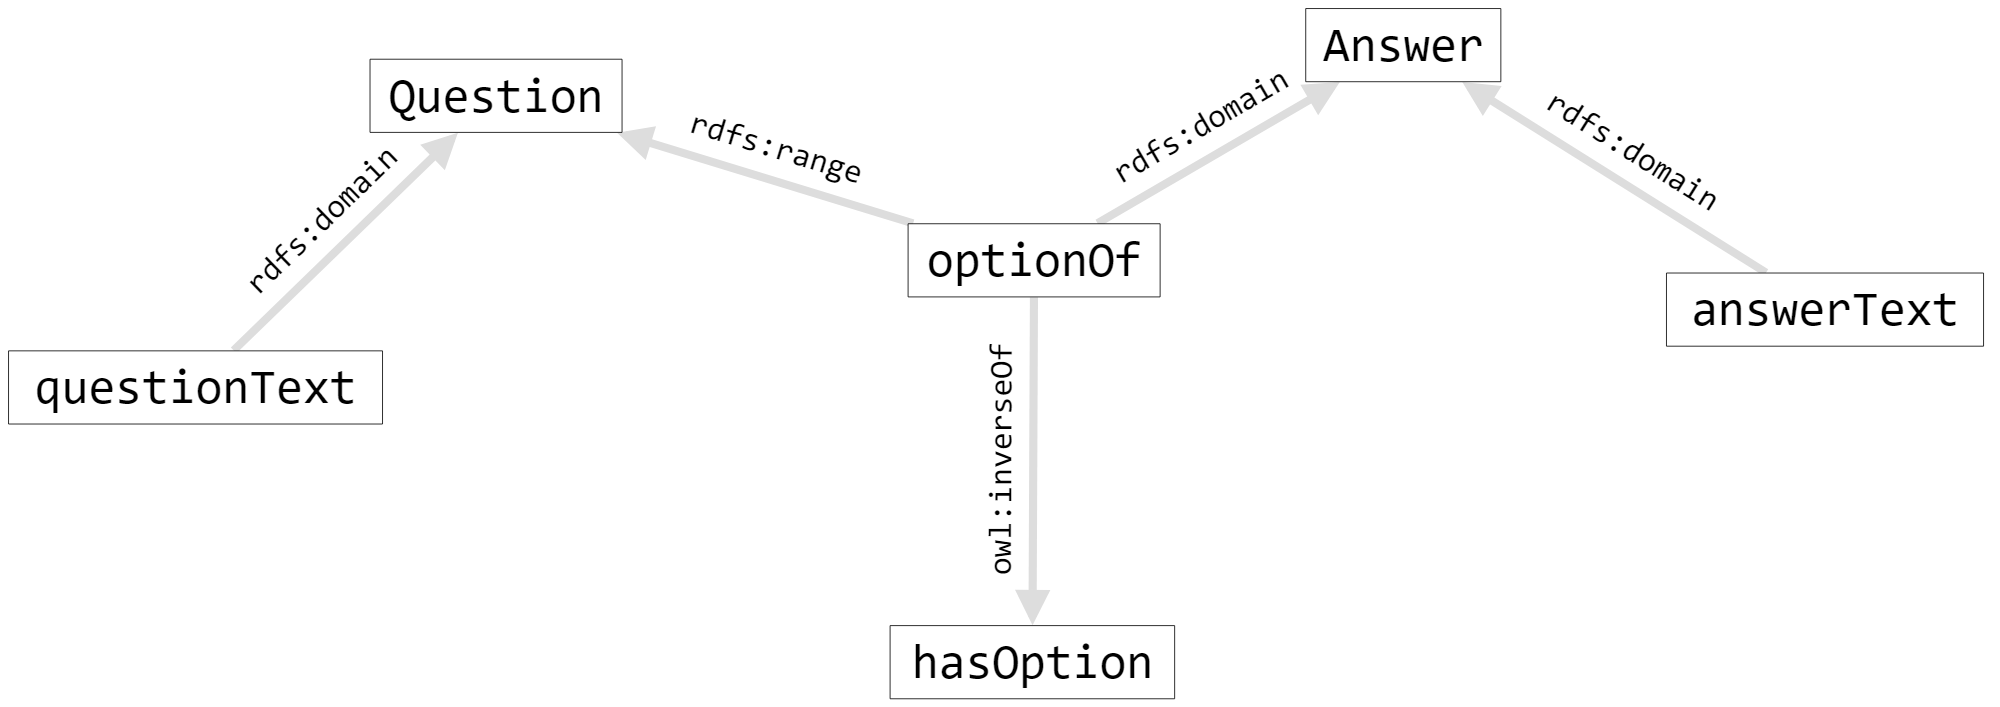
\includegraphics[width=5in]{SWWOv3/media/ch12/figure12-1.png}
\caption{Question, answer, and the properties that describe them.}
\label{fig:ch12.01}
\end{figure}



A particular questionnaire will have questions and answers. For now, we
will start with a simple questionnaire that might be part of the
screening for the helpdesk of a cable television and Internet provider:

\begin{itemize}
\item What system are you having trouble with?
\begin{itemize}
\item Possible answers (3): Cable TV, High-Speed Internet, Both
\end{itemize}

\item What television symptom(s) are you seeing?
\begin{itemize}
\item Possible answers (4): No Picture, No Sound, Tiling, Bad Reception.
\end{itemize}
\end{itemize}


This is shown as follows and graphically in Figure~\ref{fig:ch12.02}.

\begin{lstlisting}
d:WhatProblem a q:Question ;
              q:hasOption d:STV, d:SInternet, d:SBoth;  
	      q:questionText "What system are you having trouble with?" .
d:STV a q:Answer ;
              q:answerText "Cable TV" .
d:SInternet a q:Answer ;
              q:answerText "High-speed Internet" .
d:SBoth a q:Answer ;
              q:answerText "Both" .
d:TVsymptom a q:Question ;
              q:questionText "What television symptoms are you having?" ;
              q:hasOption d:TVSnothing, d:TVSnosound, d:TVStiling, d:TVSreception .
d:TVSnothing a q:Answer ;
              q:answerText "No Picture" .
d:TVSnosound a q:Answer ;
              q:answerText "No Sound".  
d:TVStiling a q:Answer ;
              q:answerText "Tiling" .
d:TVSreception a q:Answer ;
              q:answerText "Bad reception" .
\end{lstlisting}

\begin{figure}
\centering
(a)
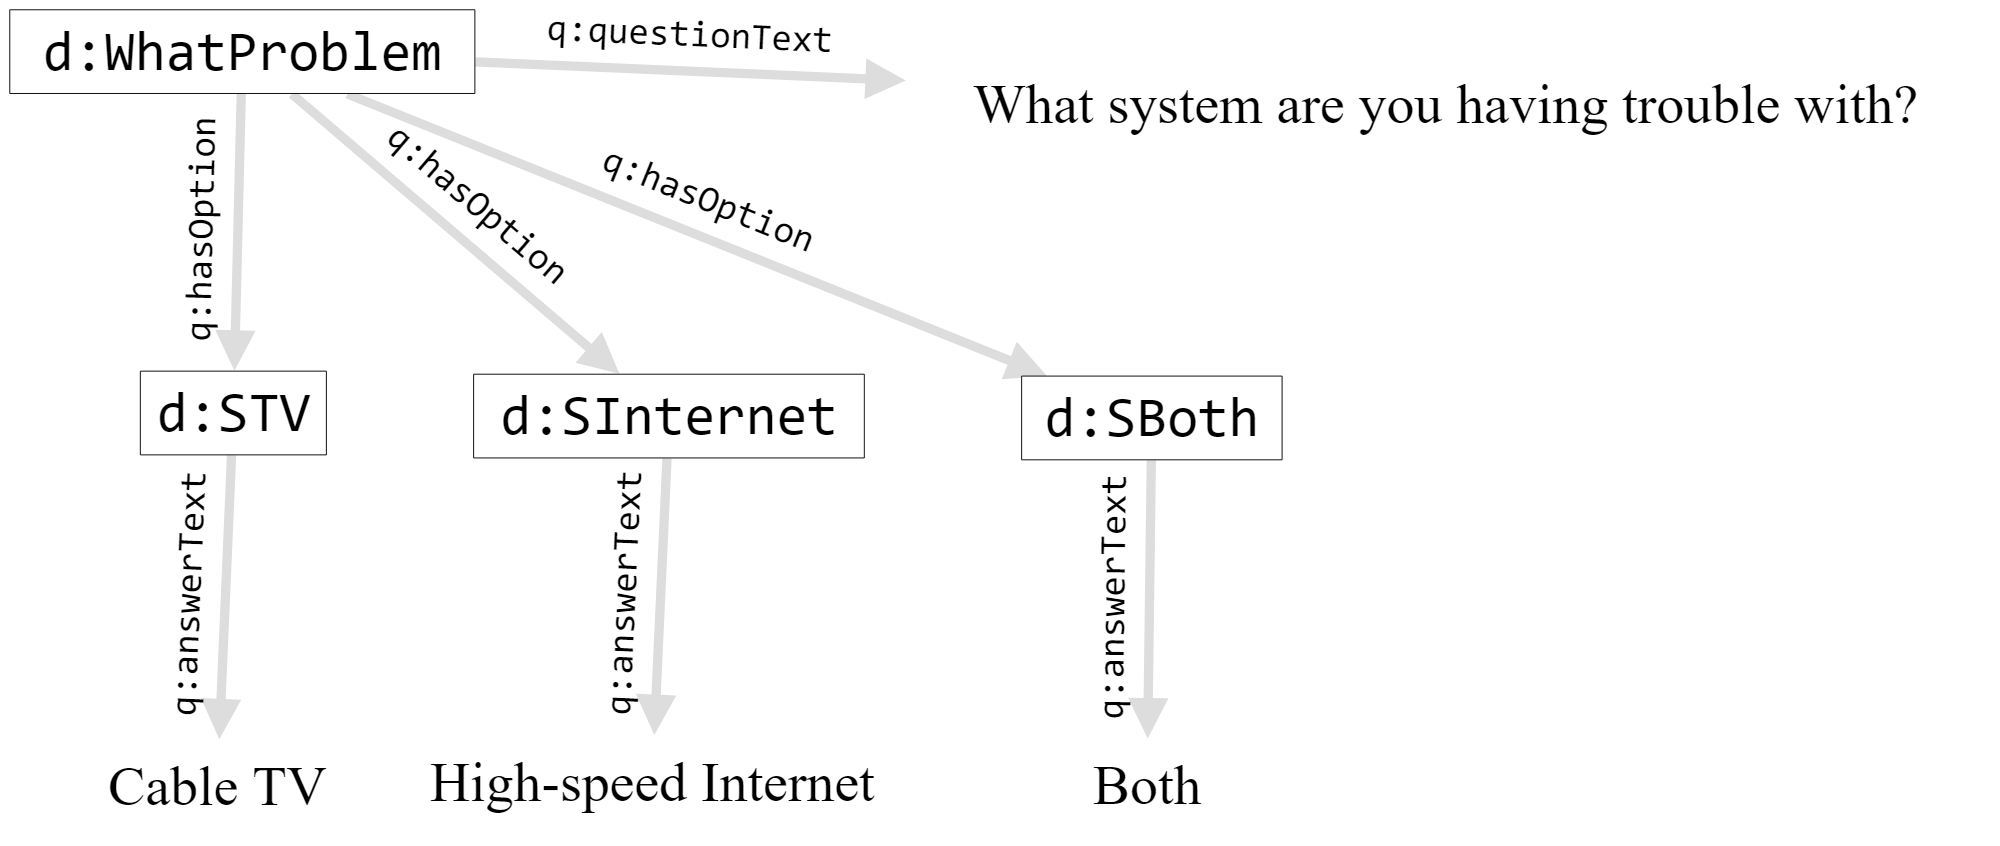
\includegraphics[width=5in]{SWWOv3/media/ch12/figure12-2a.png}
(b)
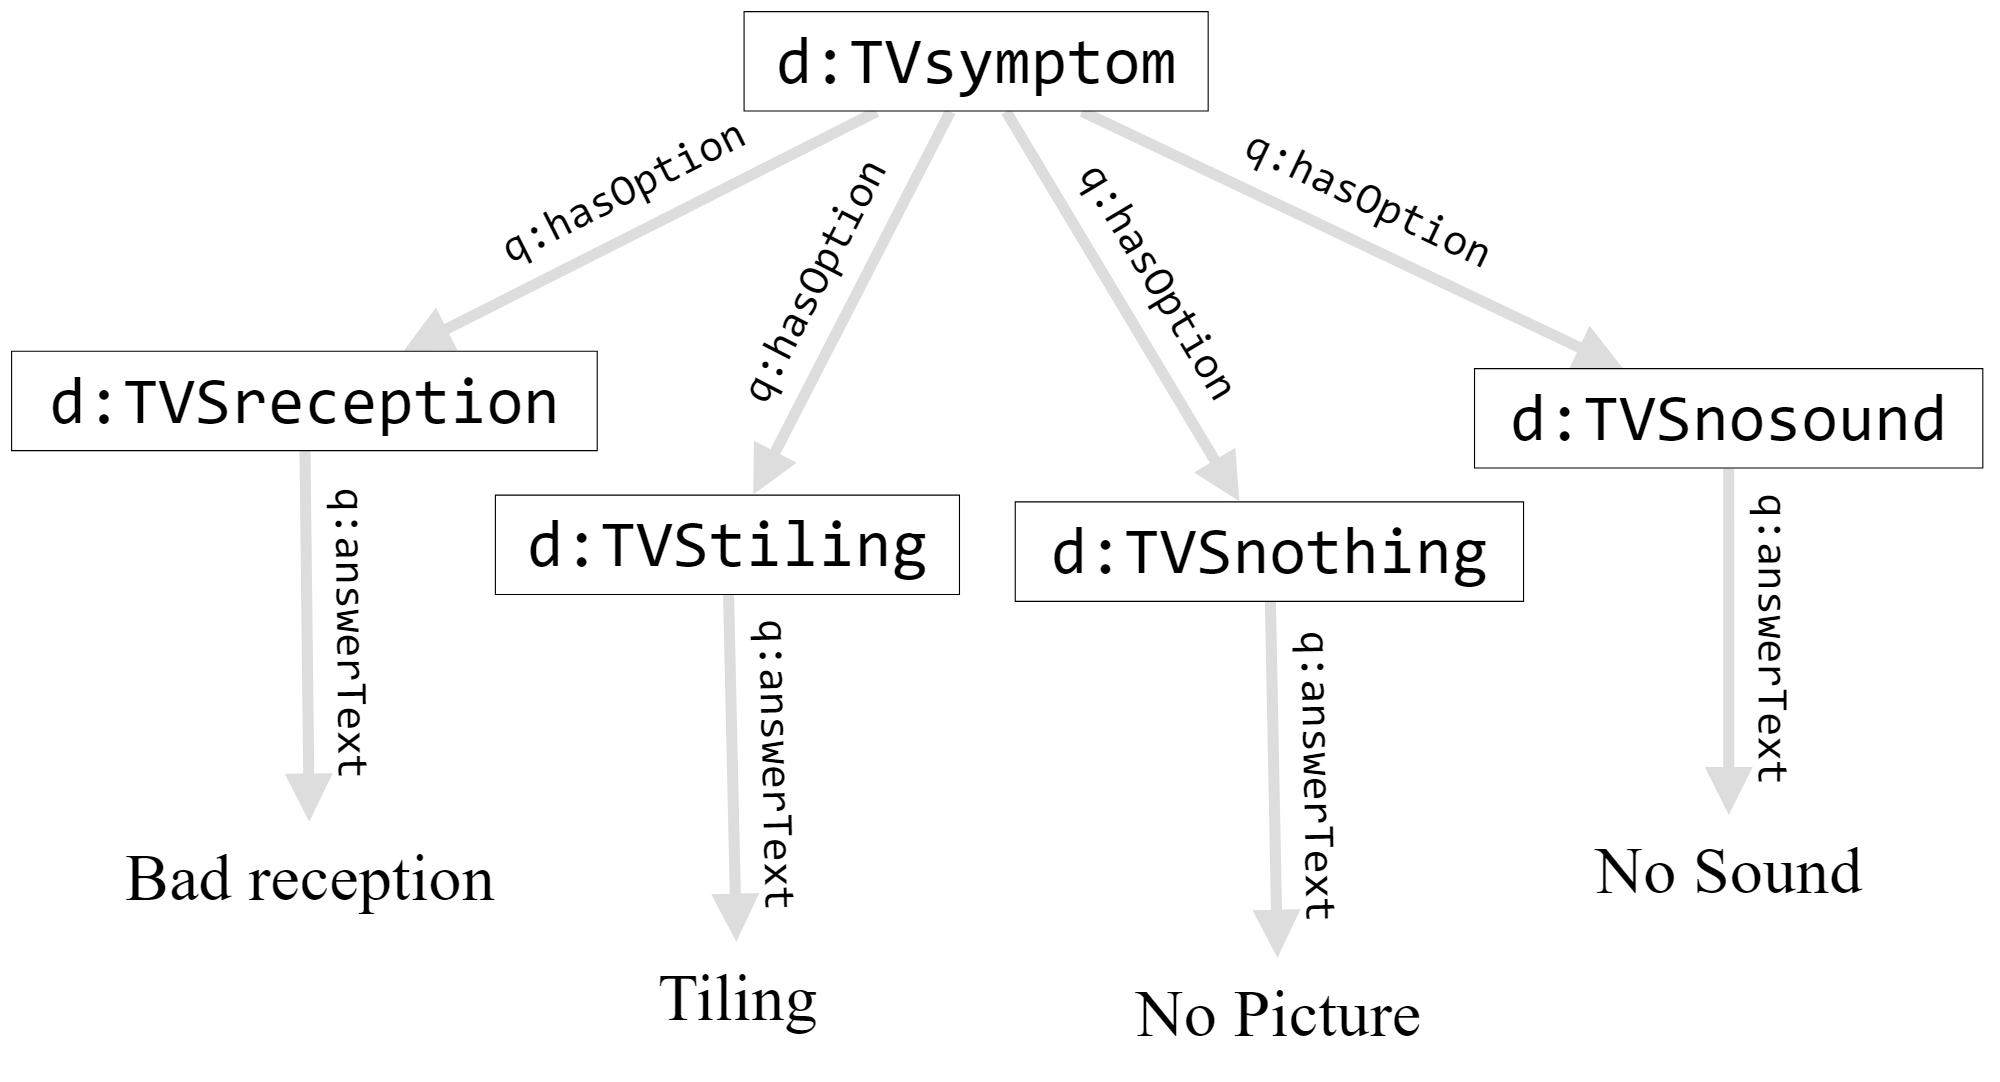
\includegraphics[width=5in]{SWWOv3/media/ch12/figure12-2b.png}
\caption{Some particular questions and their answers.}
\label{fig:ch12.02}
\end{figure}



Consider an application for managing a questionnaire in a web portal.
This application performs a query against this combined data to
determine what question(s) to ask next. Then for each question, it
presents the text of the question itself and the text of each answer,
with a \emph{select} widget (e.g., radio button) next to it. We haven't yet
defined enough information for such an application to work, and we have
made no provisions to determine which questions to ask before any others
or how to record answers to the questions. We start with the latter.

We first define a new property \texttt{hasSelectedOption}, a subproperty of
\texttt{hasOption}:

\begin{lstlisting}
q:hasSelectedOption a owl:ObjectProperty;
rdfs:subPropertyOf q:hasOption.
\end{lstlisting}

When the user who is taking a questionnaire answers a question, a new
triple will be entered to indicate that a particular option for that
question has been selected. That is, if the user selects ``Cable TV''
from the options of the first question \texttt{d:WhatProblem}, then the
application will add the triple

\begin{lstlisting}
d:WhatProblem q:hasSelectedOption d:STV.
\end{lstlisting}

to the triple store. Notice that there is no need to remove any triples
from the triple store; the original \texttt{d:hasOption} relationship between
d:WhatProblem and d:STV still holds. As we develop the example, the
model will provide ever-increasing guidance for how the selection of
questions will be done.

\end{example}

\subsection{Adding ``restrictions''}

The language construct in OWL for creating new class descriptions based
on descriptions of the prospective members of a class is called the
\emph{restriction} (\texttt{owl:Restriction}). An \texttt{owl:Restriction} is a special kind of
\emph{class}, that is, 

\begin{lstlisting}
owl:Restriction  rdfs:subClassOf owl:Class .
\end{lstlisting}

A restriction is a class that is defined by a description of its members
in terms of existing properties and classes.

In OWL, as in RDF, the AAA slogan holds: Anyone can say Anything about
Any topic. Hence, the class of all things in owl (\texttt{owl:Thing}) is
unrestricted. A \texttt{Restriction} is defined by providing some description
that limits (or \emph{restricts}) the kinds of things that can be said about a
member of the class. So if we have a property \texttt{orbitsAround}, it is
perfectly legitimate to say that anything \texttt{orbitsAround} anything else. If
we restrict the value of \texttt{orbitsAround} by saying that its object must be
\texttt{TheSun}, then we have defined the class of all things that orbit around
the sun (i.e., our solar system).

\subsection{Kinds of restrictions}
\label{ch12.restriction}
OWL provides a number of kinds of restrictions, three of which are
\texttt{owl:allValuesFrom}, \texttt{owl:someValuesFrom}, and \texttt{owl:hasValue}. Each describes
how the new class is constrained by the possible asserted values of
properties.

Additionally, a restriction class in OWL is defined by the keyword
\texttt{owl:onProperty}. This specifies what property is to be used in the
definition of the restriction class. For example, the restriction
defining the objects that orbit around the sun will use \texttt{owl:onProperty}
\texttt{orbitsAround}, whereas the restriction defining major league players will
use \texttt{owl:onProperty} \texttt{playsFor}.

A restriction is a special kind of a class, so it has individual members
just like any class.
Membership in a restriction class must satisfy the conditions specified
by the kind of restriction (\texttt{owl:allValuesFrom}, \texttt{owl:someValuesFrom}, or
\texttt{owl:hasValue}), as well as the \texttt{onProperty} specification.

\subsubsection{owl:someValuesFrom}
\label{ch12.somevaluesfrom}
\texttt{owl:someValuesFrom} is used to produce a restriction of the form ``All
individuals for which at least one value of the property P comes from
class C.'' In other words, one could define the class
\texttt{AllStarPlayer} as ``All individuals for which at least one value of the
property \texttt{playsFor} comes from the class \texttt{AllStarTeam}.'' This is what the
restriction looks like:

\begin{lstlisting}
[ a owl:Restriction;
  owl:onProperty :playsFor; 
  owl:someValuesFrom :AllStarTeam ]
\end{lstlisting}

Notice the use of the {[} \ldots{} {]} notation. As a reminder from
Chapter~\ref{ch3}, this refers to an anonymous node (a bnode) described by the
properties listed here; that is, this refers to a single bnode, which is
the subject of three triples, one per line (separated by semicolons).

The restriction class defined in this way refers to exactly the class of
individuals that satisfy these conditions on \texttt{playsFor} and \texttt{AllStarTeam}.
In particular, if an individual actually has some value from the class
\texttt{AllStarTeam} for the property \texttt{playsFor}, then it is a member of this
restriction class. Note that this restriction class, unlike those we've
learned about in earlier chapters, has no specific name associated with
it. It is defined by the properties of the restriction (i.e.,
restrictions on the members of the class) and thus it is sometimes
referred to in the literature as an ``unnamed class'' or an ``anonymous class''.

\begin{example}{Answered Questions}

In the questionnaire example, we addressed the issue of recording
answers to questions by defining a property \texttt{hasOption} that relates a
question to answer options and a subproperty \texttt{hasSelectedOption} to
indicate those answers that have been selected by the individual who is
taking the questionnaire. Now we want to address the problem of
selecting which question to ask.

There are a number of considerations that go into such a selection, but
one of them is that (under most
circumstances) we do not want to ask a question for which we already
have an answer. This suggests a class of questions that have already
been answered. We will define the set of AnsweredQuestions in terms of
the properties we have already defined. Informally, an answered question
is any question that has a selected option.

An answered question is one that has some value from the class \texttt{Answer}
for the property
\texttt{hasSelectedOption}. This can be defined as follows:

\begin{lstlisting}
q:AnsweredQuestion owl:equivalentClass
       [ a owl:Restriction ;
         owl:onProperty q:hasSelectedOption ;
         owl:someValuesFrom q:Answer ] .
\end{lstlisting}

Since

\begin{lstlisting}
d:WhatProblem q:hasSelectedOption d:STV.
\end{lstlisting}

and

\begin{lstlisting}
d:STV a q:Answer.
\end{lstlisting}

are asserted triples, the individual \texttt{d:WhatProblem} satisfies the
conditions defined by the restriction class. That is, there is at least
one value (someValue) for the property \texttt{hasSelectedOption} that is
in the class \texttt{Answer}. Individuals that satisfy the conditions specified
by a restriction class are inferred to be members of it. This inference
can be represented as follows:

\begin{lstlisting}
d:WhatProblem a [ a owl:Restriction ;
                  owl:onProperty q:hasSelectedOption ;
                  owl:someValuesFrom q:Answer ] .
\end{lstlisting}

and, thus, according to the semantics of equivalentClass,

\begin{lstlisting}
d:WhatProblem a q:AnsweredQuestion.
\end{lstlisting}
\end{example}

These definitions and inferences are shown in Figure\ref{fig:ch12.03}.

\subsubsection{owl:allValuesFrom}

\texttt{owl:allValuesFrom} is used to produce a restriction class of the form
``the individuals for which all values of the property P come from class
C.'' This restriction looks like the following:

\begin{lstlisting}
[ a owl:Restriction; 
  owl:onProperty P;
  owl:allValuesFrom C ]
\end{lstlisting}

The restriction class defined in this way refers to exactly the class of
individuals that satisfy these conditions on P and C. If an individual x
is a member of this allValuesFrom restriction, a number of conclusions
can follow, one for each triple describing x with property P. In
particular, every value of property P for individual x is inferred to be
in class C. So, if My Favorite All Star Team is restricted to all players being star players, then every player on my favorite all star team is a star player.  Furthermore, if Kaneda and Gonzales play on my favorite all star team, then both of them must be star players.  This intuition is shown in triples below (with the usual convention that inferred triples are marked with an asterisk (*):

\begin{lstlisting}
MyFavoriteAllStarTeam a BaseballTeam ;
                      a [ owl:Restriction ;
		                  owl:onProperty :hasPlayer ;
		             	  owl:allValuesFrom :StarPlayer ] ;
                      :hasPlayer :Kaneda, :Gonzales .
* :Gonzales a :StarPlayer .
* :Kaneda a :StarPlayer .
\end{lstlisting}



\begin{figure}
\centering
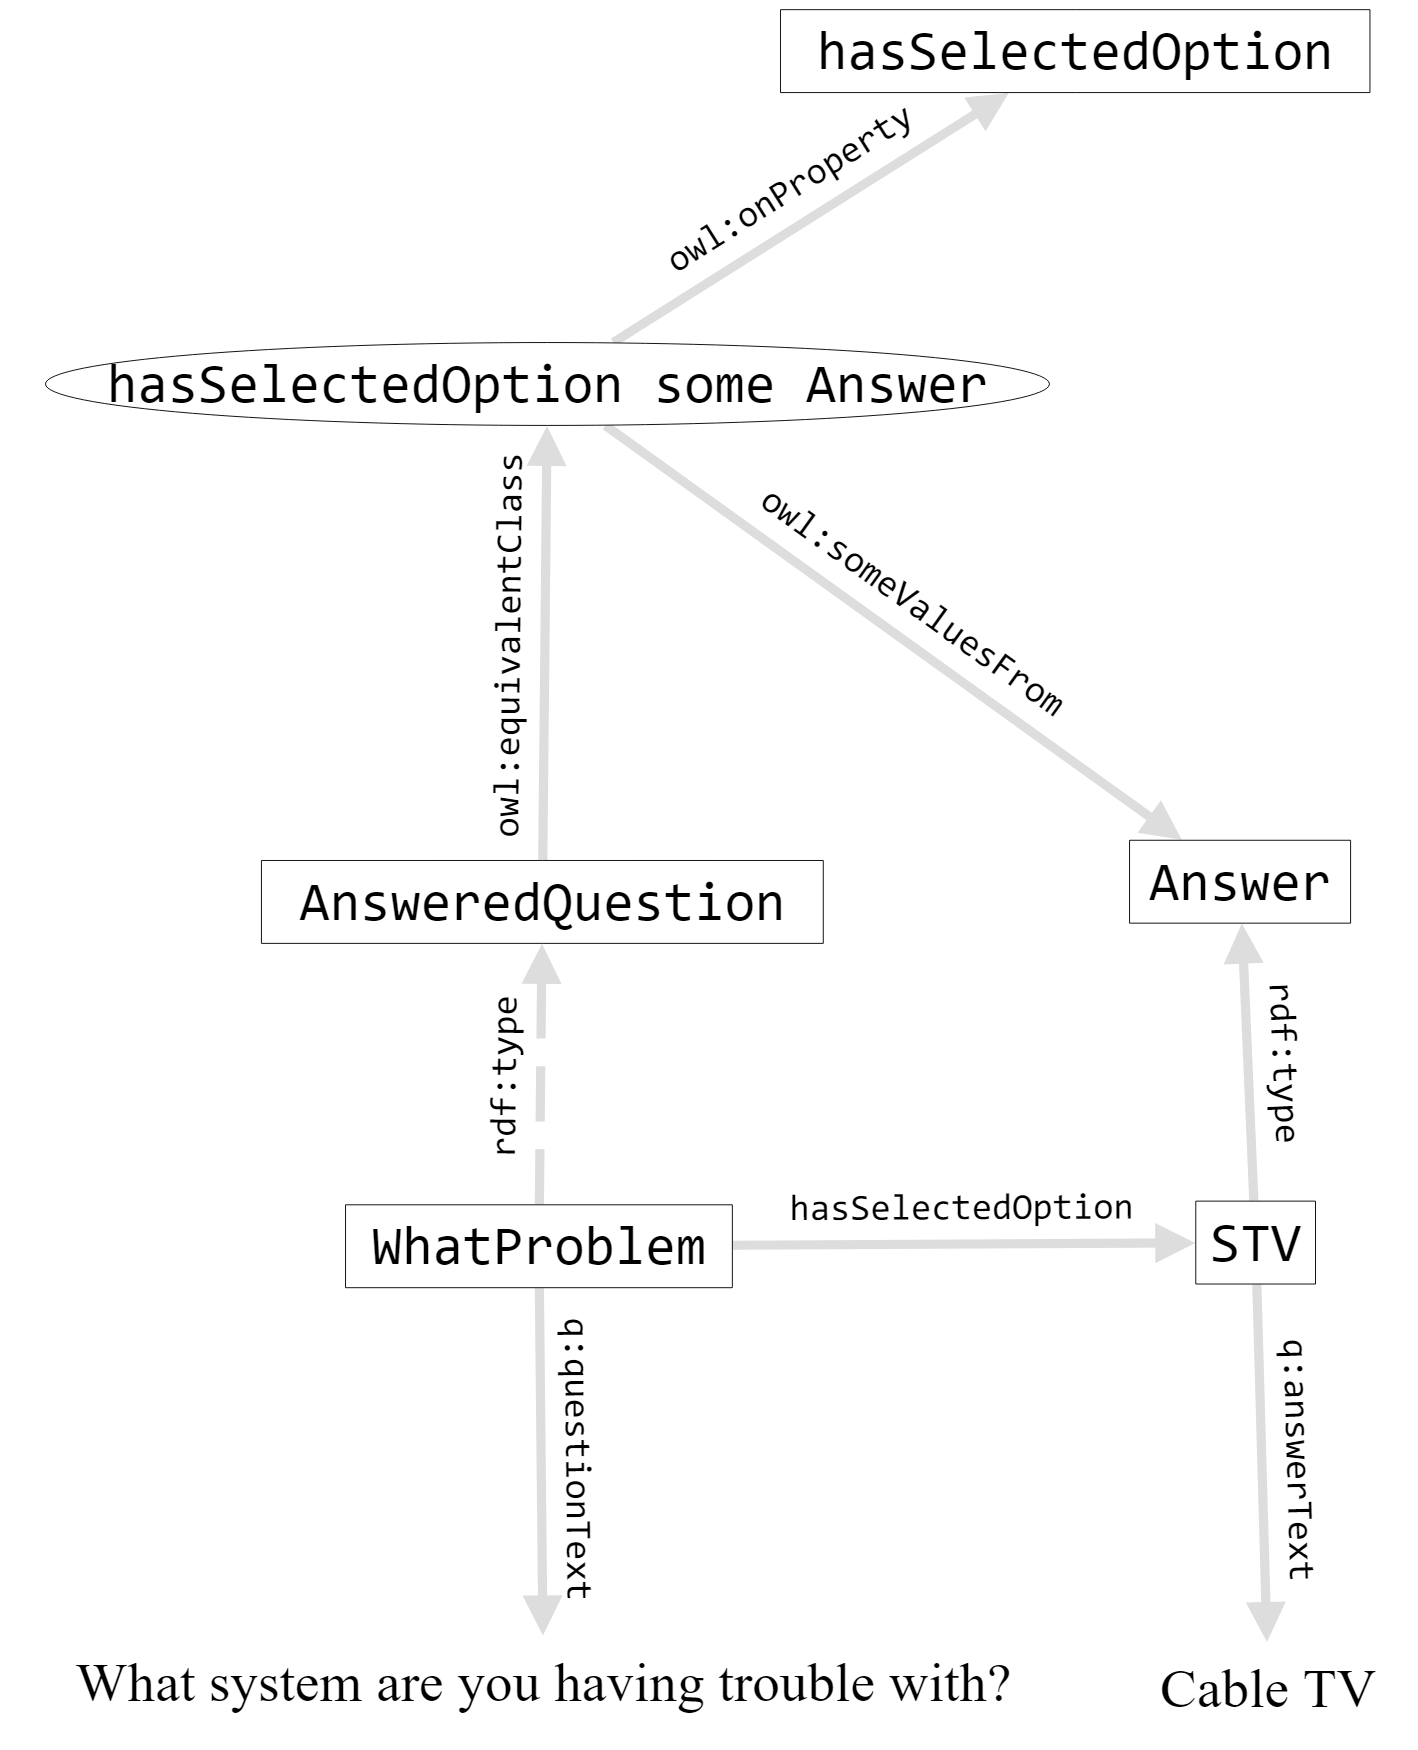
\includegraphics[width=5in]{SWWOv3/media/ch12/figure12-3.png}
\caption{Definition of \texttt{q:AnsweredQuestion} and the resulting inferences for
\texttt{d:WhatProblem}. Since \texttt{d:WhatProblem} has something (\texttt{d:STV}) of type
\texttt{q:Answer} on property \texttt{q:hasSelectedOption}, it is inferred (dotted line)
to be a member of \texttt{AnsweredQuestion}.
}
\label{fig:ch12.03}
\end{figure}





There is a subtle difference between \texttt{someValuesFrom} and \texttt{allValuesFrom}.
Since
\texttt{someValuesFrom} is defined as a restriction class such that there is at
least one member of a class with a particular property, then it implies
that there must be such a member. On the other hand, \texttt{allValuesFrom}
technically means ``if there are any members, then they all must have
this property.'' This latter does not imply that there are any members.
This will be more important in later chapters.

\begin{example}{Question Dependencies}

In our questionnaire example, we might want to ask certain questions
only after particular answers have been given. To accomplish this, we
begin by defining the class of all selected answers, based on the
property \texttt{hasSelectedOption} we have already defined. We can borrow a
technique from Chapter\ref{ch8} to do this. First, we define a class for the
selected answers:

\begin{lstlisting}
q:SelectedAnswer a owl:Class;
                 rdfs:subClassOf q:Answer.
\end{lstlisting}

We want to ensure that any option that has been selected will appear in
this class. This can be done easily by asserting that

\begin{lstlisting}
q:hasSelectedOption rdfs:range q:SelectedAnswer.
\end{lstlisting}

This ensures that any value V that appears as the object of a triple of
the form

\begin{lstlisting}
? q:hasSelectedOption V.
\end{lstlisting}

is a member of the class \texttt{SelectedAnswer}. In particular, since we have
asserted that

\begin{lstlisting}
d:WhatProblem q:hasSelectedOption d:STV.
\end{lstlisting}

we can infer that

\begin{lstlisting}
d:STV a q:SelectedAnswer.
\end{lstlisting}

\end{example}

Now that we have defined the class of selected answers, we describe the
questions that can be asked only after those answers have been given. We
introduce a new class called EnabledQuestion; only questions that also
have type EnabledQuestion are actually available to be asked:

\begin{lstlisting}
q:EnabledQuestion a owl:Class.
\end{lstlisting}

When an answer is selected, we want to infer that certain dependent
questions become members of
\texttt{EnabledQuestion}. This can be done with an \texttt{owl:allValuesFrom} restriction.

To begin, each answer potentially makes certain questions available for
asking. We define a property called \texttt{enablesCandidate} for this
relationship. In particular, we say that an answer enables a question if
selecting that answer causes the system to consider that question as a
candidate for the next question to ask:

\begin{lstlisting}
q:enablesCandidate a owl:ObjectProperty ;
                   rdfs:domain q:Answer ;
                   rdfs:range q:Question .
\end{lstlisting}

In our example, we only want to ask a question about television problems
if the answer to the first question indicates that there is a television
problem:

\begin{lstlisting}
d:STV q:enablesCandidate d:TVsymptom .
d:SBoth q:enablesCandidate d:TVsymptom .
\end{lstlisting}

That is, if the answer to the first question, ``What system are you
having trouble with?,'' is either ``Cable TV'' or ``Both,'' then we want
to be able to ask the question ``What television symptoms are you
having?''

The following \texttt{owl:allValuesFrom} restriction does just that: It defines
the class of things all of
whose values for \texttt{d:enablesCandidate} come from the class
\texttt{d:EnabledQuestion}:

\begin{lstlisting}
[ a owl:Restriction ;
  owl:onProperty q:enablesCandidate ;
  owl:allValuesFrom q:EnabledQuestion ]
\end{lstlisting}

Which answers should enforce this property? We only want this for the
answers that have been selected. How do we determine which answers have
been selected? So far, we only have the property \texttt{hasSelectedOption} to
indicate them. That is, for any member of \texttt{SelectedAnswer}, we want it to
also be a member of this restriction class. This is exactly what the
relation \texttt{rdfs:subClassOf} does for us:

\begin{lstlisting}
q:SelectedAnswer rdfs:subClassOf
        [ a owl:Restriction ;
          owl:onProperty q:enablesCandidate ;
          owl:allValuesFrom q:EnabledQuestion] .
\end{lstlisting}

That is, a selected answer is a subclass of the unnamed restriction
class.

Let's watch how this works, step by step. When the user selects the
answer ``Cable TV'' for the first question, the type of \texttt{d:STV} is
asserted to be SelectedAnswer, like the preceding.

\begin{lstlisting}
d:STV a q:SelectedAnswer .
\end{lstlisting}

However, because of the rdfs:subClassOf relation, \texttt{d:STV} is a member of
the restriction class, that is, it has the restriction as its type:

\begin{lstlisting}
d:STV a
       [ a owl:Restriction ;
         owl:onProperty q:enablesCandidate ;
         owl:allValuesFrom q:EnabledQuestion ] .
\end{lstlisting}

Any individual who is a member of this restriction necessarily satisfies
the \texttt{allValuesFrom} condition; that is, any individual that it is related
to by
\texttt{d:enablesCandidate} must be a member of \texttt{d:EnabledQuestion}. Since

\begin{lstlisting}
d:STV q:enablesCandidate d:TVsymptom .
\end{lstlisting}

we can infer that

\begin{lstlisting}
* d:TVsymptom a q:EnabledQuestion .
\end{lstlisting}

as desired. Finally, since we have also asserted the same information
for the answer \texttt{d:SBoth},

\begin{lstlisting}
d:SBoth q:enablesCandidate d:TVsymptom.
\end{lstlisting}

We can see this inference and the triples that led to it in Figure~\ref{fig:ch12.04}


\begin{figure}
\centering
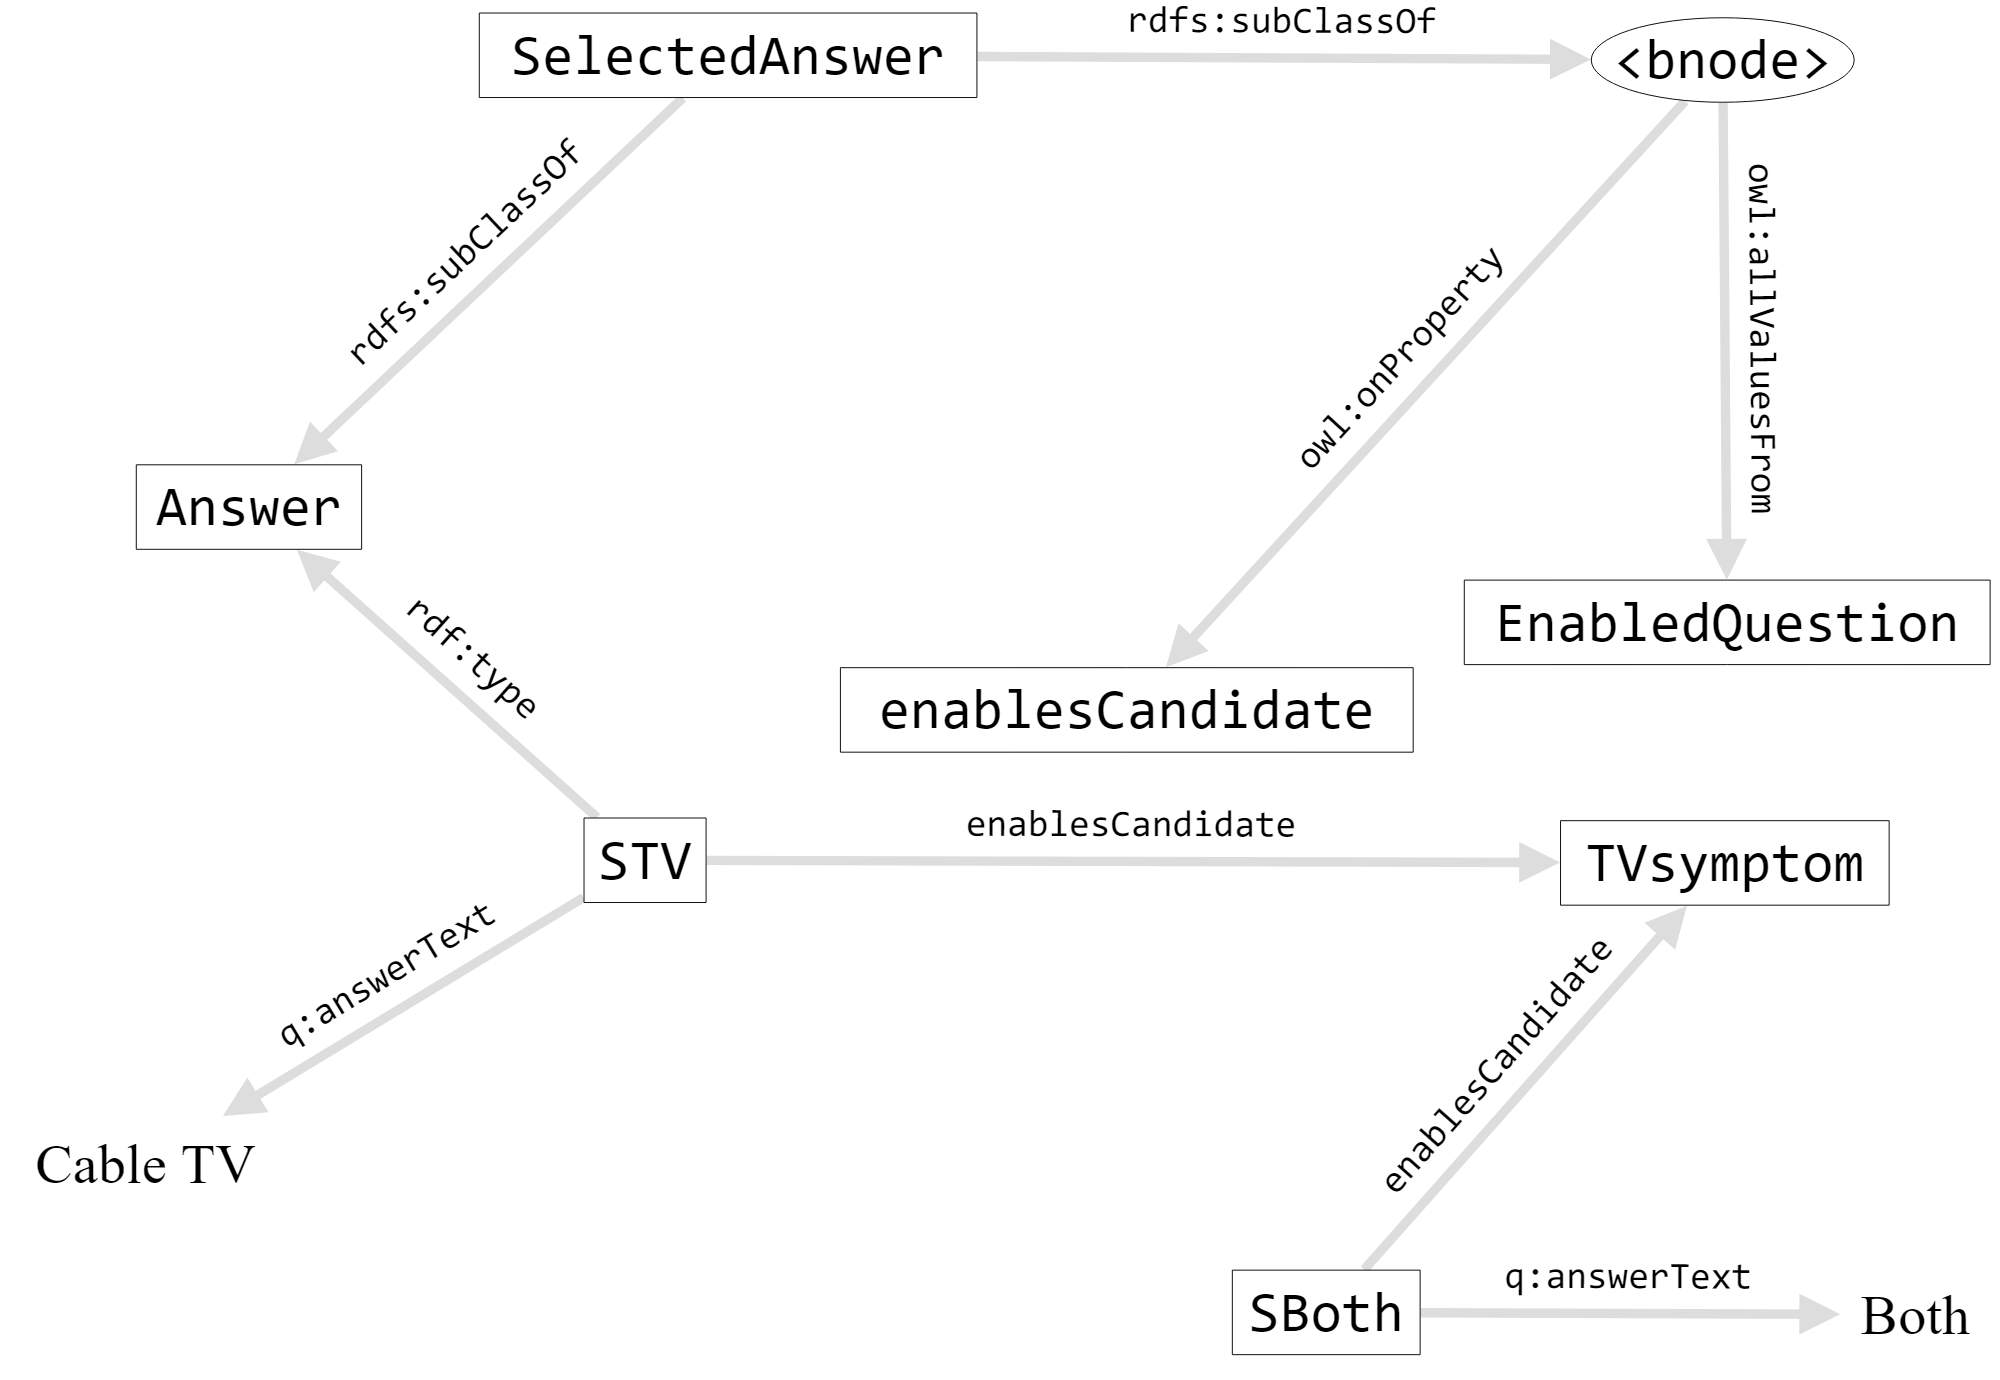
\includegraphics[width=5in]{SWWOv3/media/ch12/figure12-4.png}
\caption{\texttt{d:STV} \texttt{enablesCandidate} \texttt{TVSymptom}, but it is also a member of a
restriction on the property \texttt{enablesCandidate}, stipulating that all
values must come from the class \texttt{q:EnabledQuestion}. We can therefore
infer that \texttt{d:TVSymptom} has type \texttt{q:EnabledQuestion}. 
}
\label{fig:ch12.04}
\end{figure}



\begin{figure}
\centering
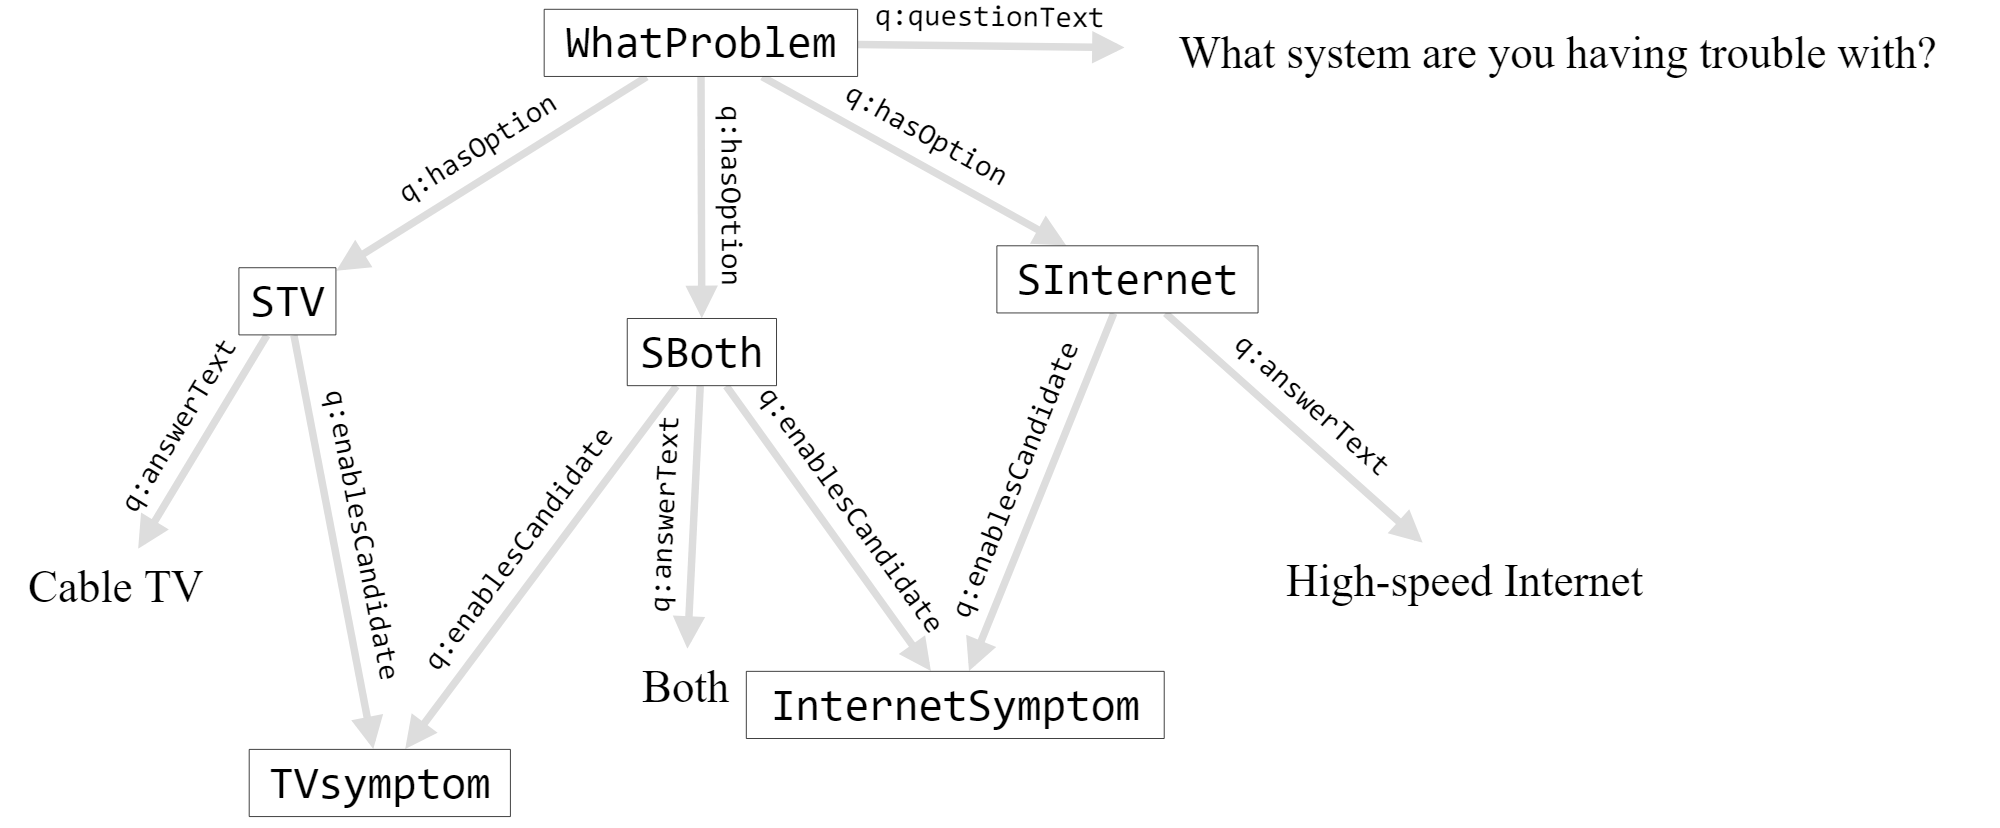
\includegraphics[width=5in]{SWWOv3/media/ch12/figure12-5.png}
\caption{Questions and the answers that enable them.}
\label{fig:ch12.05}
\end{figure}



Since \texttt{SBoth} also enables the candidate \texttt{TVSymptom}, the same conclusion
will be drawn if the user answers ``Both'' to the first question. If we
were to extend the example with another question about Internet symptoms
\texttt{d:InternetSymptom}, then we could express all the dependencies in this
short questionnaire as follows:

\begin{lstlisting}
d:STV q:enablesCandidate d:TVsymptom .
d:SBoth q:enablesCandidate d:TVsymptom .
d:SBoth q:enablesCandidate d:InternetSymptom .
d:SInternet q:enablesCandidate d:InternetSymptom .
\end{lstlisting}

The dependency tree is shown graphically in Figure~\ref{fig:ch12.05}.

\begin{example}{Prerequisites}

In the previous example, we supposed that when we answered one question,
it made all of its dependent questions eligible for asking. Another way
questions are related to one another in a questionnaire is a
prerequisite. If a question has a number of prerequisites, all of them
must be answered appropriately for the question to be eligible.

Consider the following triples that define a section of a questionnaire:

\begin{lstlisting}
d:NeighborsToo a q:Question ;
               q:hasOption d:NTY, d:NTN, d:NTDK ;
               q:questionText "Are other customers in your 
                               building also experiencing
                               problems?" .
d:NTY a q:Answer ;
               q:answerText "Yes, my neighbors are 
                             experiencing the same problem."  .
d:NTN a q:Answer ;
               q:answerText "No, my neighbors are not 
                             experiencing the same problem." .
d:NTDK a q:Answer ;
               q:answerText "I don't know." .
\end{lstlisting}

This question makes sense only if the current customer lives in a
building with other customers and is experiencing a technical problem.
That is, this question depends on the answers to two more questions,
shown following. The answer to the first question (\texttt{d:othersinbuilding})
should be \texttt{d:OYes}, and the answer to the second question (\texttt{d:whatissue})
should be \texttt{d:PTech}:

\begin{lstlisting}
d:othersinbuilding
       a q:Question ;
       q:hasOption d:ONo, d:OYes ;
       q:questionText
           "Do you live in a multi-unit dwelling 
            with other customers?" .
d:OYes a q:Answer ;
       q:answerText "Yes." .
d:ONo a q:Answer ;
       q:answerText "No." .
d:whatIssue
       a q:Question ;
       q:hasOption d:PBilling, d:PNew, d:PCancel,
                   d:PTech;
       q:questionText
          "What can customer service help you with today?" .
d:PBilling a q:Answer ;
       q:answerText "Billing question." .
d:PNew a q:Answer ;
       q:answerText "New account" .
d:PCancel a q:Answer ;
       q:answerText "Cancel account".  
d:PTech a q:Answer ;
       q:answerText "Technical difficulty" .
\end{lstlisting}

A graphic version of these questions can be seen in Figure~\ref{fig:ch12.06}.
\end{example}
\begin{figure}
\centering
(a)
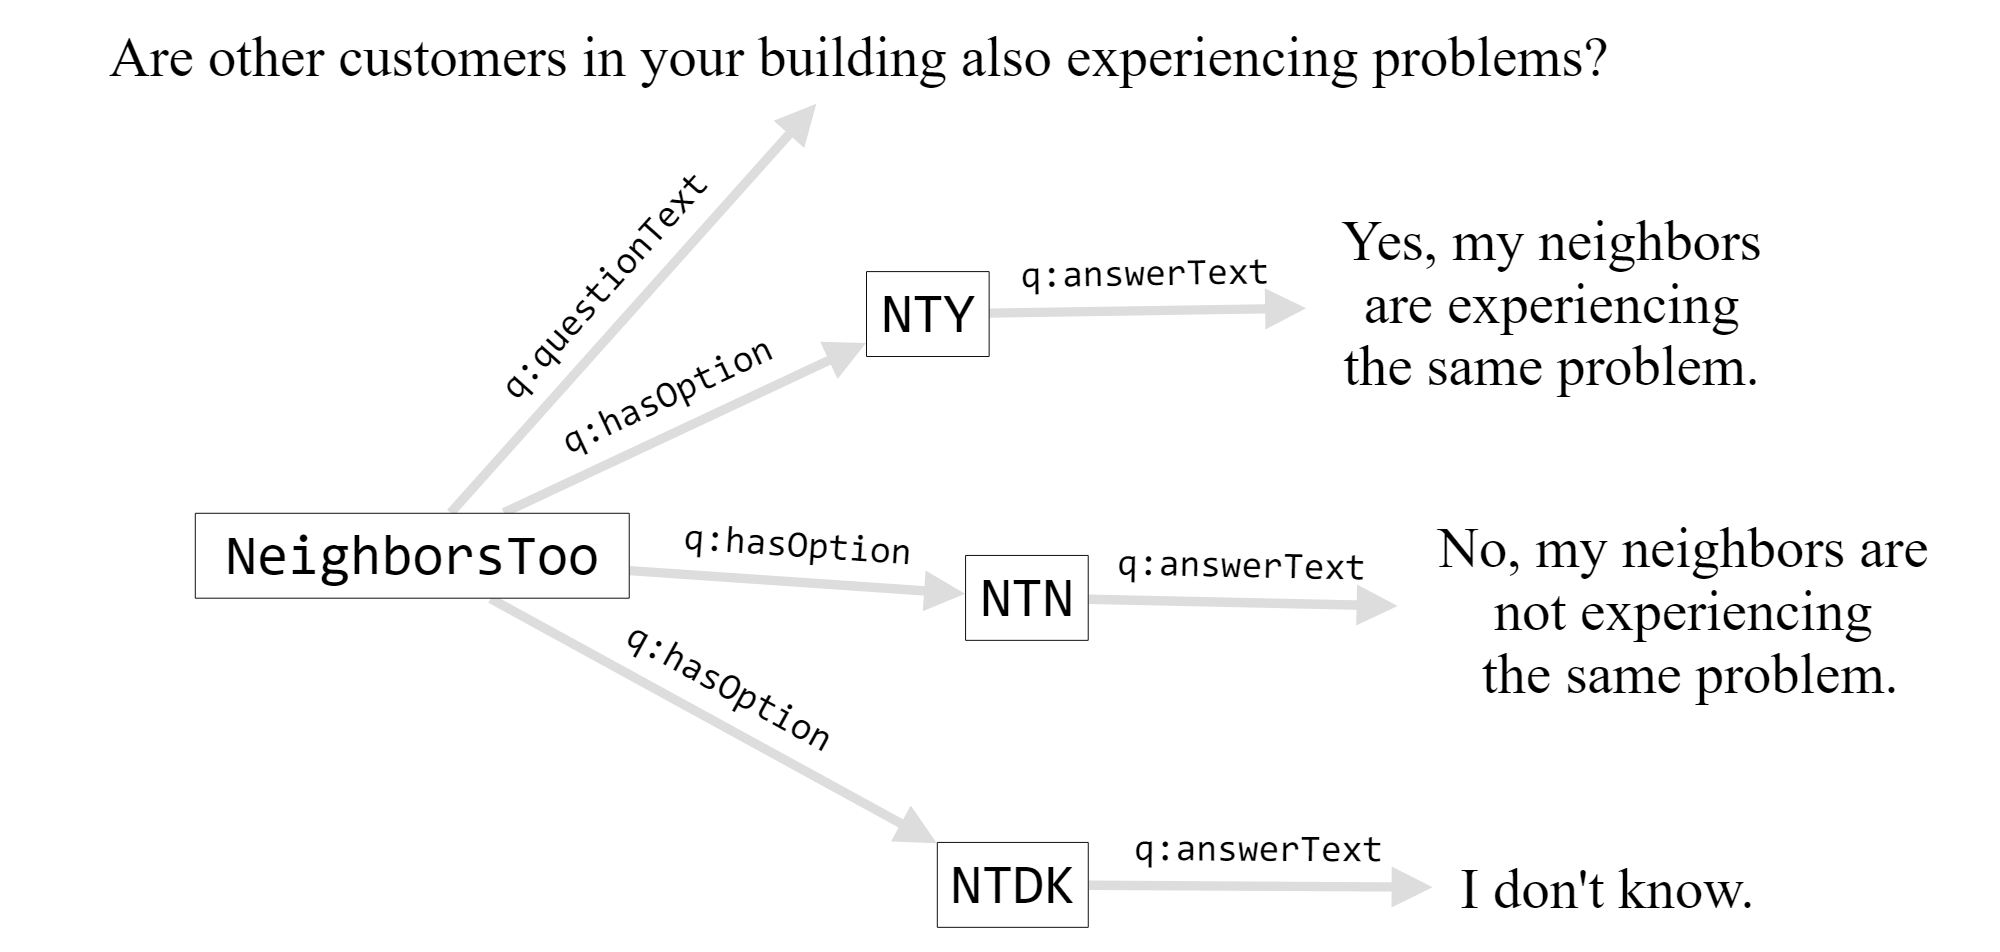
\includegraphics[width=5in]{SWWOv3/media/ch12/figure12-6a.png}
(b)
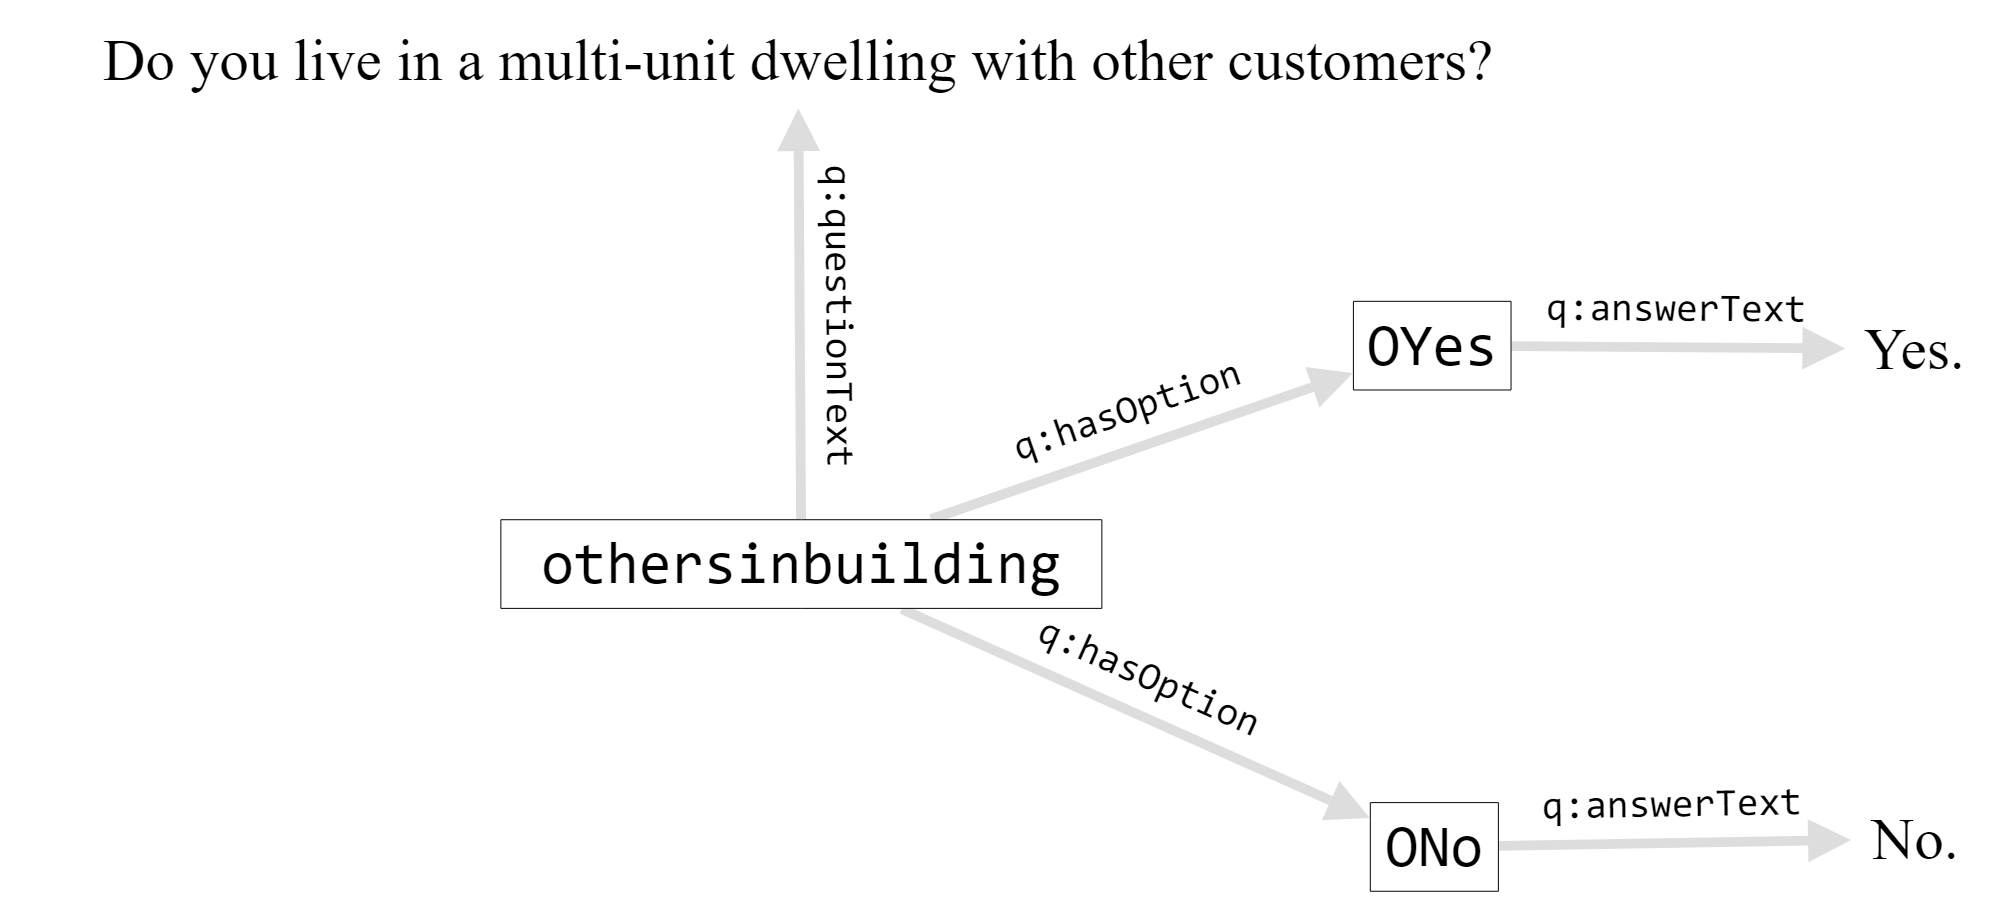
\includegraphics[width=5in]{SWWOv3/media/ch12/figure12-6b.png}
(c)
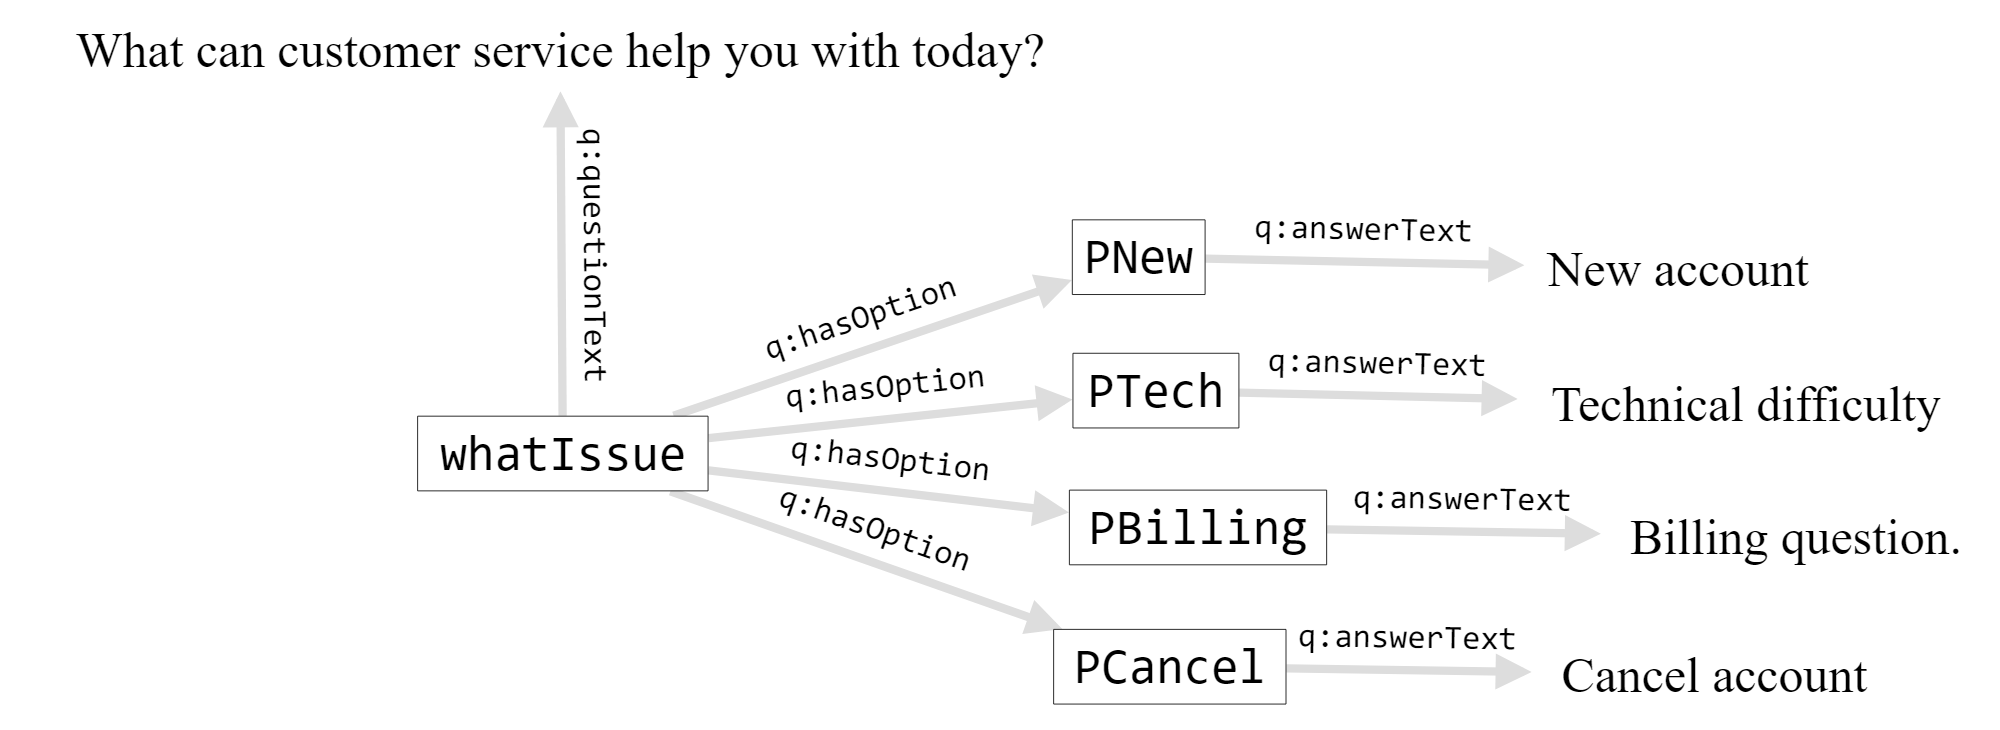
\includegraphics[width=5in]{SWWOv3/media/ch12/figure12-6c.png}
\caption{Questions about neighbors have two prerequisite questions.}
\label{fig:ch12.06}
\end{figure}

\begin{challenge}{Restricted selection}
\label{chal:26}

How can we model the relationship between \texttt{d:NeighborsToo}, \texttt{d:whatIssue},
and \texttt{d:othersinbuilding} so that we will only ask \texttt{d:NeighborsToo} when we
have appropriate answers to both d:whatIssue and d:othersinbuilding?

We introduce a new property \texttt{q:hasPrerequisite} that will relate a
question to its prerequisites:

\begin{lstlisting}
q:hasPrerequisite rdfs:domain q:Question; rdfs:range q:Answer.
\end{lstlisting}

We can indicate the relationship between the questions using this
property:

\begin{lstlisting}
d:NeighborsToo q:hasPrerequisite d:PTech, d:OYes.
\end{lstlisting}

This prerequisite structure is shown in graphical form in Figure~\ref{fig:ch12.07}.

Now we want to say that we will infer something is a \texttt{d:EnabledQuestion}
if all of its prerequisite answers are selected. We begin by asserting
that

\begin{figure}
\centering
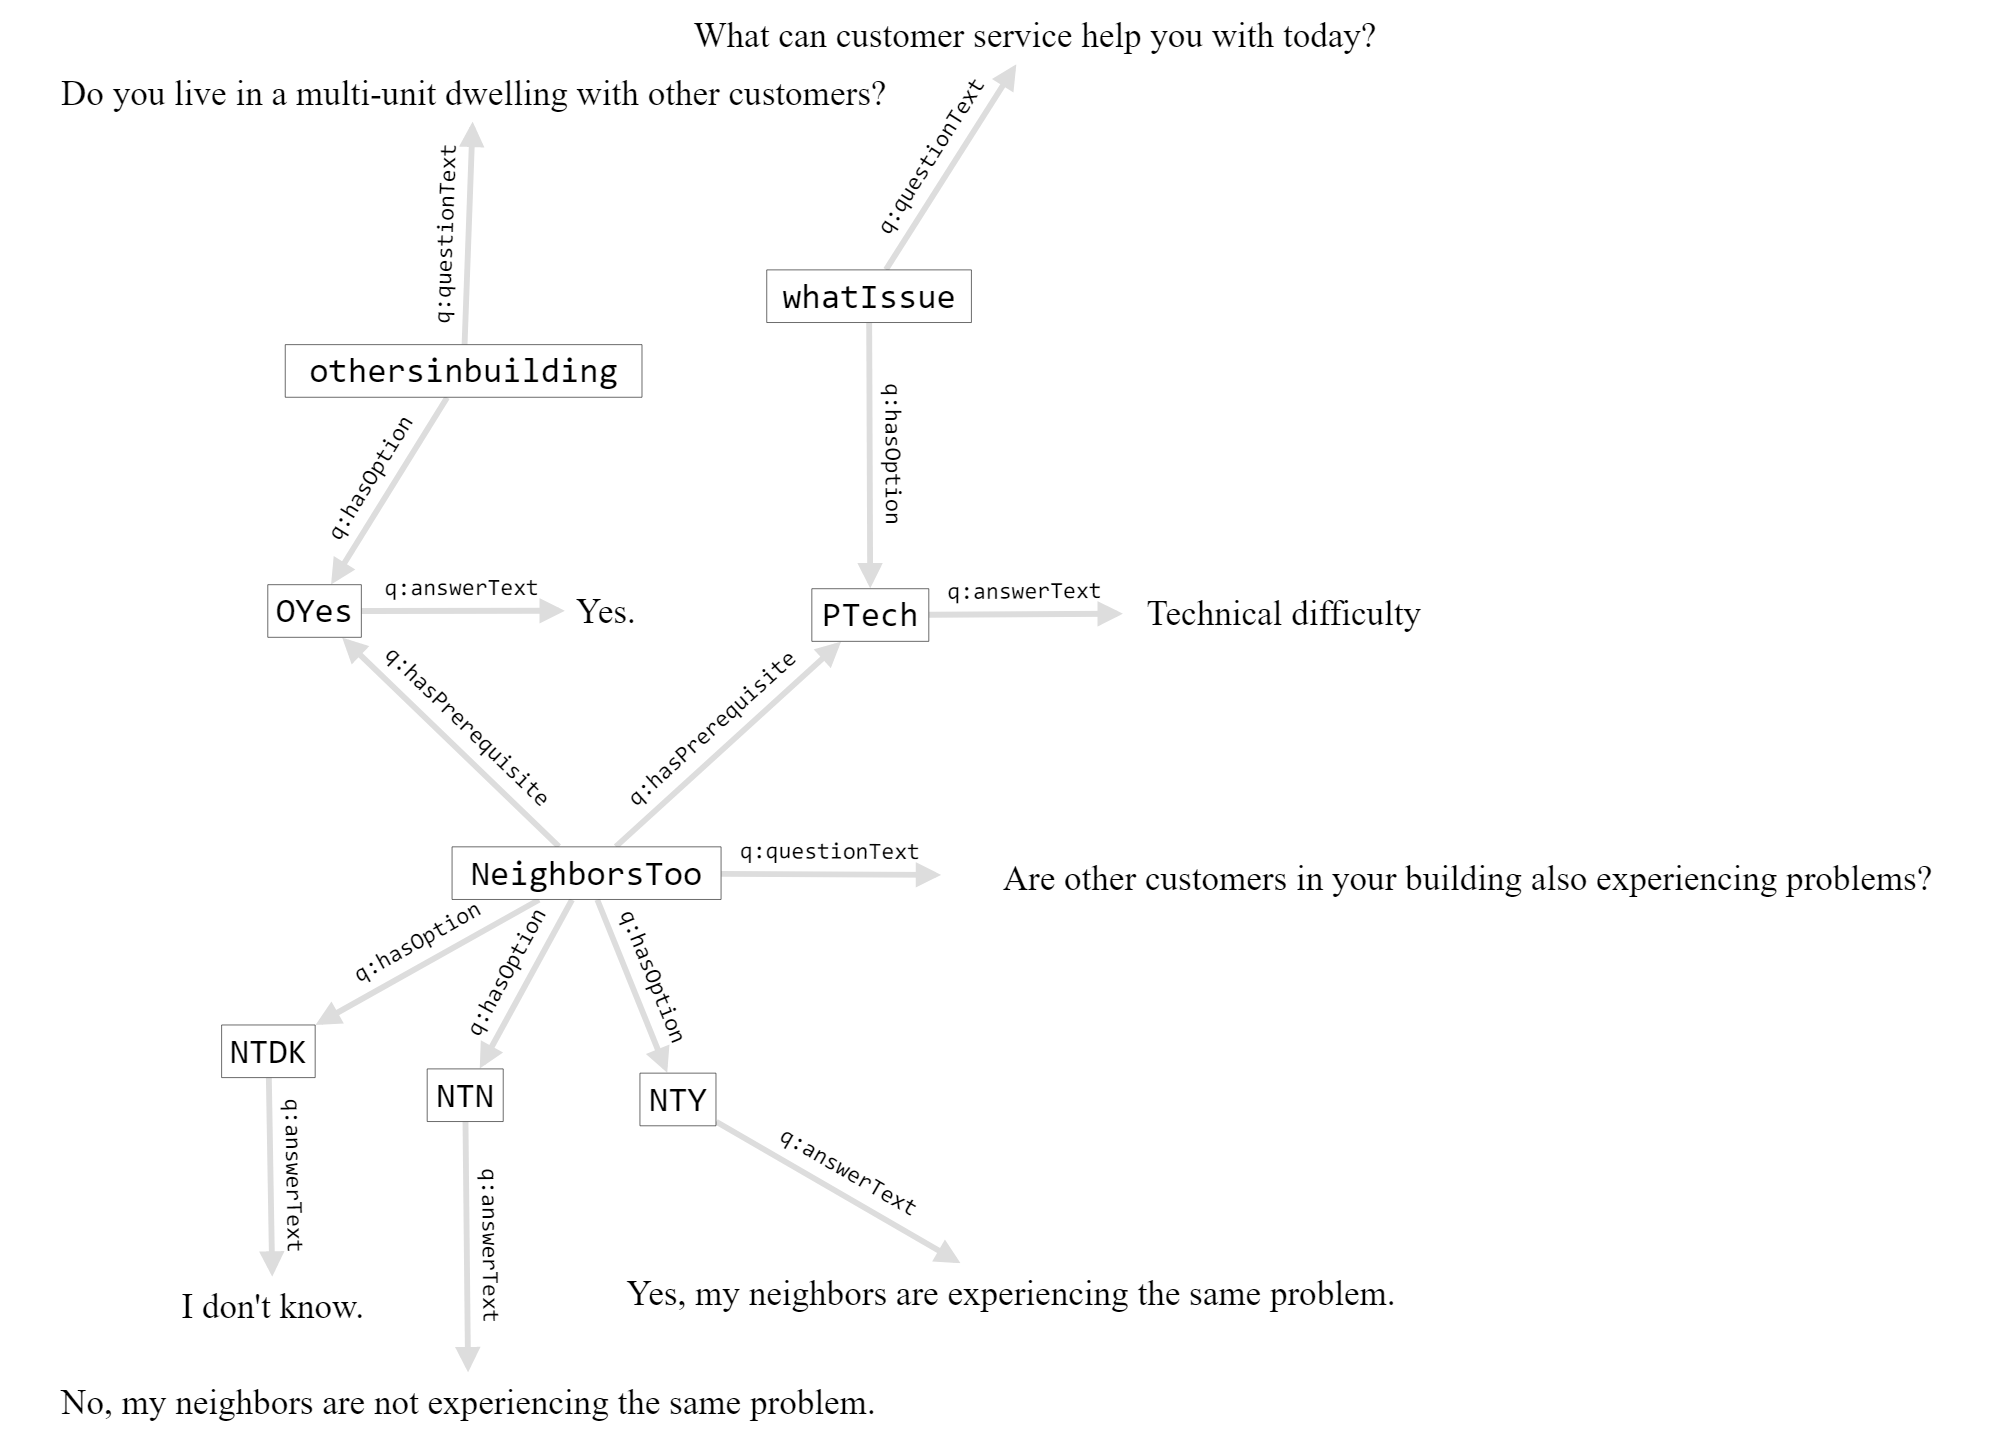
\includegraphics[width=5in]{SWWOv3/media/ch12/figure12-7.png}
\caption{Some questions and their prerequisites.}
\label{fig:ch12.07}
\end{figure}


\begin{lstlisting}
[ a owl:Restriction ;
  owl:onProperty q:hasPrerequisite ;
  owl:allValuesFrom q:SelectedAnswer ]
 rdfs:subClassOf q:EnabledQuestion .
\end{lstlisting}

Notice that we can use the restriction class just as we could any other
class in OWL, so in this case we have said that the restriction is a
subclass of another class. Any question that satisfies the restriction
will be inferred to be a member of d:EnabledQuestion by this subclass
relation. But how can we infer that something satisfies this
restriction?

For an individual \texttt{?x} to satisfy this restriction, we must know that
every time there is a triple of the form

\begin{lstlisting}
?x hasPrerequisite ?y.
\end{lstlisting}

\texttt{?y} must be a member of the class \texttt{d:SelectedAnswer}. But by the Open World
Assumption, we don't know if there might be another triple of this form
for which \texttt{?y} is not a member of \texttt{d:SelectedAnswer}. Given the Open World
assumption, how can we ever know that all prerequisites have been met?
\end{challenge}

The rest of this challenge will have to wait until we discuss the
various methods by which we can (partially) close the world in OWL. The
basic idea is that if we can say how many prerequisites a question has,
then we can know when all of them have been selected. If we know that a
question has only one prerequisite, and we find one that it is
satisfied, then it must be the one. If we know that a question has no
prerequisites at all, then we can determine that it is an
\texttt{EnabledQuestion} without having to check for any \texttt{SelectedAnswers} at all.

\subsubsection{owl:hasValue}

The third kind of restriction in OWL is called \texttt{owl:hasValue}. As in the
other two restrictions, it acts on a particular property as specified by
\texttt{owl:onProperty}. It is used to produce a restriction whose description is
of the form ``All individuals that have the value A for the property P''
and looks as follows:

\begin{lstlisting}
[ a owl:Restriction ;
  owl:onProperty P ;
  owl:hasValue A ]
\end{lstlisting}

Formally, the \texttt{hasValue} restriction is just a special case of the
\texttt{someValuesFrom} restriction, in which the class C happens to be a
singleton set \{A\}.

Although it is ``just'' a special case, \texttt{owl:hasValue} has been identified
in the OWL standard in its own right because it is a very common and
useful modeling form. It effectively turns specific instance
descriptions into class descriptions. For example, ``The set of all
planets orbiting the sun'' and ``The set of all baseball teams in
Japan'' are defined using hasValue restrictions.

\begin{example}{Priority Questions}

Suppose that in our questionnaire, we assign priority levels to our
questions. First we define a class of priority levels and particular
individuals that define the priorities in the questionnaire:

\begin{lstlisting}
q:PriorityLevel a owl:Class .
q:High a q:PriorityLevel .
q:Medium a q:PriorityLevel .
q:Low a q:PriorityLevel .
\end{lstlisting}

Then we define a property that we will use to specify the priority level
of a question:

\begin{lstlisting}
q:hasPriority rdfs:range q:PriorityLevel.
\end{lstlisting}
\end{example}

We have defined the range of \texttt{q:hasPriority} but not its domain. After
all, we might want to set priorities for any number of different sorts
of things, not just questions. We can use \texttt{owl:hasValue} to define the
class of high-priority items:

\begin{lstlisting}
q:HighPriorityItem owl:equivalentClass
    [ a owl:Restriction;
      owl:onProperty q:hasPriority;
      owl:hasValue q:High ].
\end{lstlisting}

These triples are shown graphically in Figure~\ref{fig:ch12.08}. Note that where
before we defined subclasses and superclasses of a restriction class,
here we use \texttt{owl:equivalentClass} to specify that these classes are the
same. So we have created a named class (\texttt{q:HighPriorityItem}) that is the
same as the unnamed restriction class, and we can use this named class
if we want to make other assertions or to further restrict the class.

We can describe Medium and Low priority questions in the same manner:

\begin{lstlisting}
q:MediumPriorityItem owl:equivalentClass
    [ a owl:Restriction ;
      owl:onProperty q:hasPriority ;
      owl:hasValue q:Medium ] .
q:LowPriorityItem owl:equivalentClass 
    [ a owl:Restriction ;
      owl:onProperty q:hasPriority ;
      owl:hasValue q:Low ] .
\end{lstlisting}

If we assert the priority level of a question, such as the following:

\begin{lstlisting}
d:WhatProblem q:hasPriority q:High .
d:InternetSymptom q:hasPriority q:Low .
\end{lstlisting}

then we can infer the membership of these questions in their respective
classes:

\begin{lstlisting}
d:WhatProblem a q:HighPriorityItem .
d:InternetSymptom a q:LowPriorityItem .
\end{lstlisting}

We can also use \texttt{owl:hasValue} to work ``the other way around.'' Suppose
we assert that \texttt{d:TVsymptom} is in the class \texttt{HighPriorityItem}:


\begin{lstlisting}
d:TVsymptom a q:HighPriorityItem.
\end{lstlisting}

Then by the semantics of \texttt{owl:equivalentClass}, we can infer that
\texttt{d:TVsymptom} is a member of the restriction class and must be bound by
its stipulations. Thus, we can infer that

\begin{lstlisting}
d:TVsymptom q:hasPriority q:High.
\end{lstlisting}


\begin{figure}
\centering
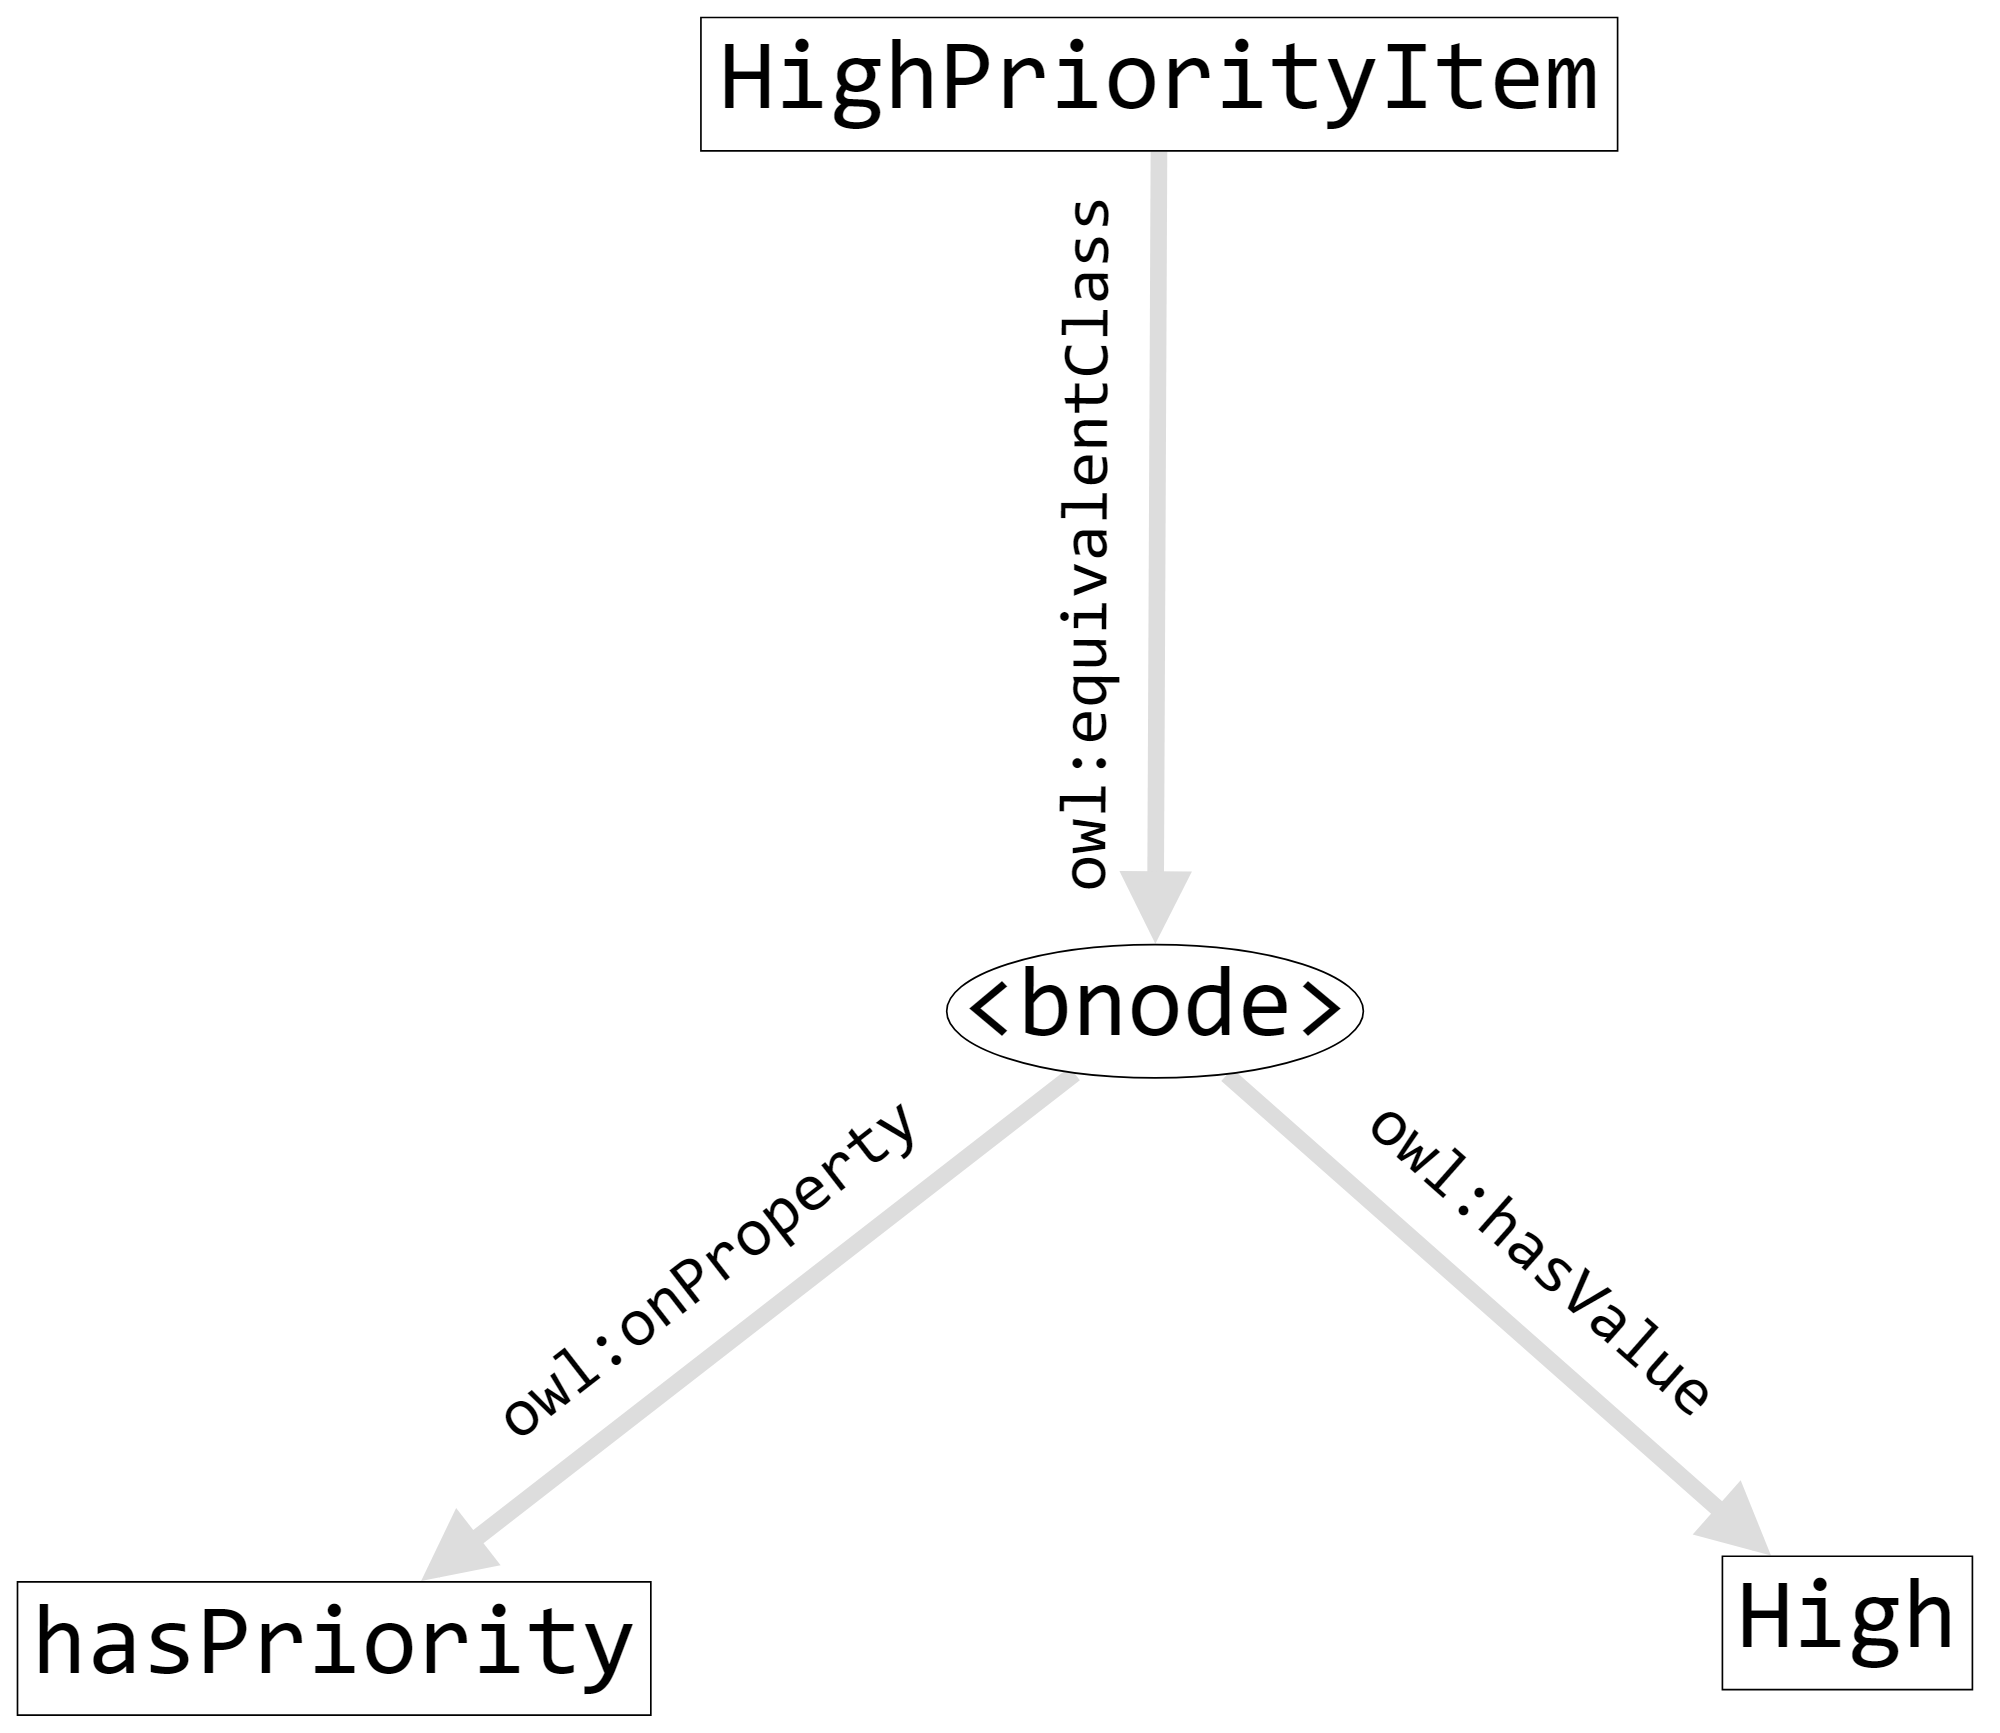
\includegraphics[width=5in]{SWWOv3/media/ch12/figure12-8.png}
\caption{Definition of a HighPriorityItem as anything that has value High for the
hasPriority property.
}
\label{fig:ch12.08}
\end{figure}



Notice that there is no stipulation in this definition to say that a
\texttt{HighPriorityItem} must be a question; after all, we might set priorities
for things other than questions. The only way we know that \texttt{d:TVsymptom}
is a \texttt{q:Question} is that we already asserted that fact. In the next
chapter, we will see how to use set operations to make definitions that
combine restrictions with other classes.

\section{Challenge Problems}

As we saw in the previous examples, the class constructors in OWL can be
combined in a wide variety of powerful ways. In this section, we present
a series of challenges that can be addressed using these OWL constructs.
Often the application of the construct is quite simple; however, we have
chosen these challenge problems because of their relevance to modeling
problems that we have seen in real modeling projects.

\subsection{Local restriction of ranges}
\label{lror}
We have already seen how \texttt{rdfs:domain} and \texttt{rdfs:range} can be used to
classify data according to how it is used. But in more elaborate
modeling situations, a finer granularity of domain and range inferences
is needed. Consider the following example of describing a vegetarian
diet:

\begin{lstlisting}
:Person a owl:Class .
:Food a owl:Class .
:eats rdfs:domain :Person .
:eats rdfs:range :Food .
\end{lstlisting}

From these triples and the following instance data

\begin{lstlisting}
:Maverick :eats :Steak.
\end{lstlisting}

we can conclude two things:

\begin{lstlisting}
* :Maverick a:Person .
* :Steak a:Food .
\end{lstlisting}

The former is implied by the domain information, and the latter by the
range information.

Suppose we want to define a variety of diets in more detail. What would
this mean? First, let's suppose that we have a particular kind of
person, called a Vegetarian, and the kind of food that a Vegetarian
eats, which we will call simply \texttt{VegetarianFood}, as subclasses of \texttt{Person}
and \texttt{Food}, respectively:

\begin{lstlisting}
:Vegetarian a owl:Class ;
            rdfs:subClassOf :Person .
:VegetarianFood a owl:Class ;
            rdfs:subClassOf :Food .
\end{lstlisting}

Suppose further that we say

\begin{lstlisting}
:Jen a :Vegetarian ;
     :eats :Hummus .
\end{lstlisting}

We would like to be able to infer that

\begin{lstlisting}
:Hummus a :VegetarianFood .
\end{lstlisting}

but not make the corresponding inference for Maverick's steak until
someone asserts that he, too, is a vegetarian.

\begin{challenge}{Restricted range with owl:Restriction}

It is tempting to represent this with more domain and range
statements---thus:

\begin{lstlisting}
:eats rdfs:domain :Vegetarian .
:eats rdfs:range :VegetarianFood .
\end{lstlisting}

But given the meaning of rdfs:domain and rdfs:range, we can draw
inferences from these triples that we do not intend. In particular, we
can infer

\begin{lstlisting}
* :Maverick a :Vegetarian .
* :Steak a :VegetarianFood .
\end{lstlisting}

which would come as a surprise both to Maverick and the vegetarians of
the world.

How can the relationship between vegetarians and vegetarian food be
correctly modeled with the use of the
owl:Restriction?

\solution

We can define the set of things that only eat VegetarianFood using a
restriction, owl:allValuesFrom; we can then assert that any Vegetarian
satisfies this condition using rdfs:subClassOf. Together, it looks like
this:

\begin{lstlisting}
:Vegetarian rdfs:subClassOf
      [ a owl:Restriction;
        owl:onProperty :eats;
        owl:allValuesFrom :VegetarianFood ] .
\end{lstlisting}

Let's see how it works. Since

\begin{lstlisting}
:Jen a :Vegetarian .
\end{lstlisting}

we can conclude that

\begin{lstlisting}
:Jen a [ a owl:Restriction ;
         owl:onProperty :eats ;
         owl:allValuesFrom :VegetarianFood ] .
\end{lstlisting}

Combined with the fact that

\begin{lstlisting}
:Jen :eats :Hummus .
\end{lstlisting}

we can conclude that

\begin{lstlisting}
:Hummus a:VegetarianFood .
\end{lstlisting}

as desired. How does Maverick fare now? We won't say that he is a
Vegetarian but only, as we have stated already, that he is a Person.
That's where the inference ends; there is no stated relationship between
Maverick and Vegetarian, so there is nothing on which to base an
inference. Maverick's steak remains simply a \texttt{Food}, not a \texttt{VegetarianFood}.

The entire model and inferences are shown in Figure~\ref{fig:ch12.09}.
\end{challenge}

\begin{challenge}{Filtering data based on explicit type}
\label{chal:27x}

We have seen how tabular data can be used in RDF by considering each row
to be an individual, the column names as properties, and the values in
the table as values. We saw sample data in Table~\ref{tab:ch3.12}, which we repeat
on  as Table~\ref{tab:ch12.1}. Some sample triples from these data are shown
in Table~\ref{tab:ch12.2}.

Each row from the original table appears in Table~\ref{tab:ch12.1} as an individual
in the RDF version. Each of these individuals has the same
type---namely, \texttt{mfg:Product}---from the name of the table. These data
include only a limited number of possible values for the
``Product\_Line'' field, and they are known in advance (e.g., ``Paper
machine,'' ``Feedback line,'' ``Safety Valve,'' etc.).

A more elaborate way to import this information would be to still have
one individual per row in the original table but to have rows with
different types depending on the value of the Product Line column. For
example, the following triples (among others) would be imported:

\begin{lstlisting}
mfg:Product1 rdf:type ns:Paper_machine .
mfg:Product4 rdf:type ns:Feedback_line .
mfg:Product7 rdf:type ns:Monitor .
mfg:Product9 rdf:type ns:SafetyValve .
\end{lstlisting}


\begin{figure}
\centering
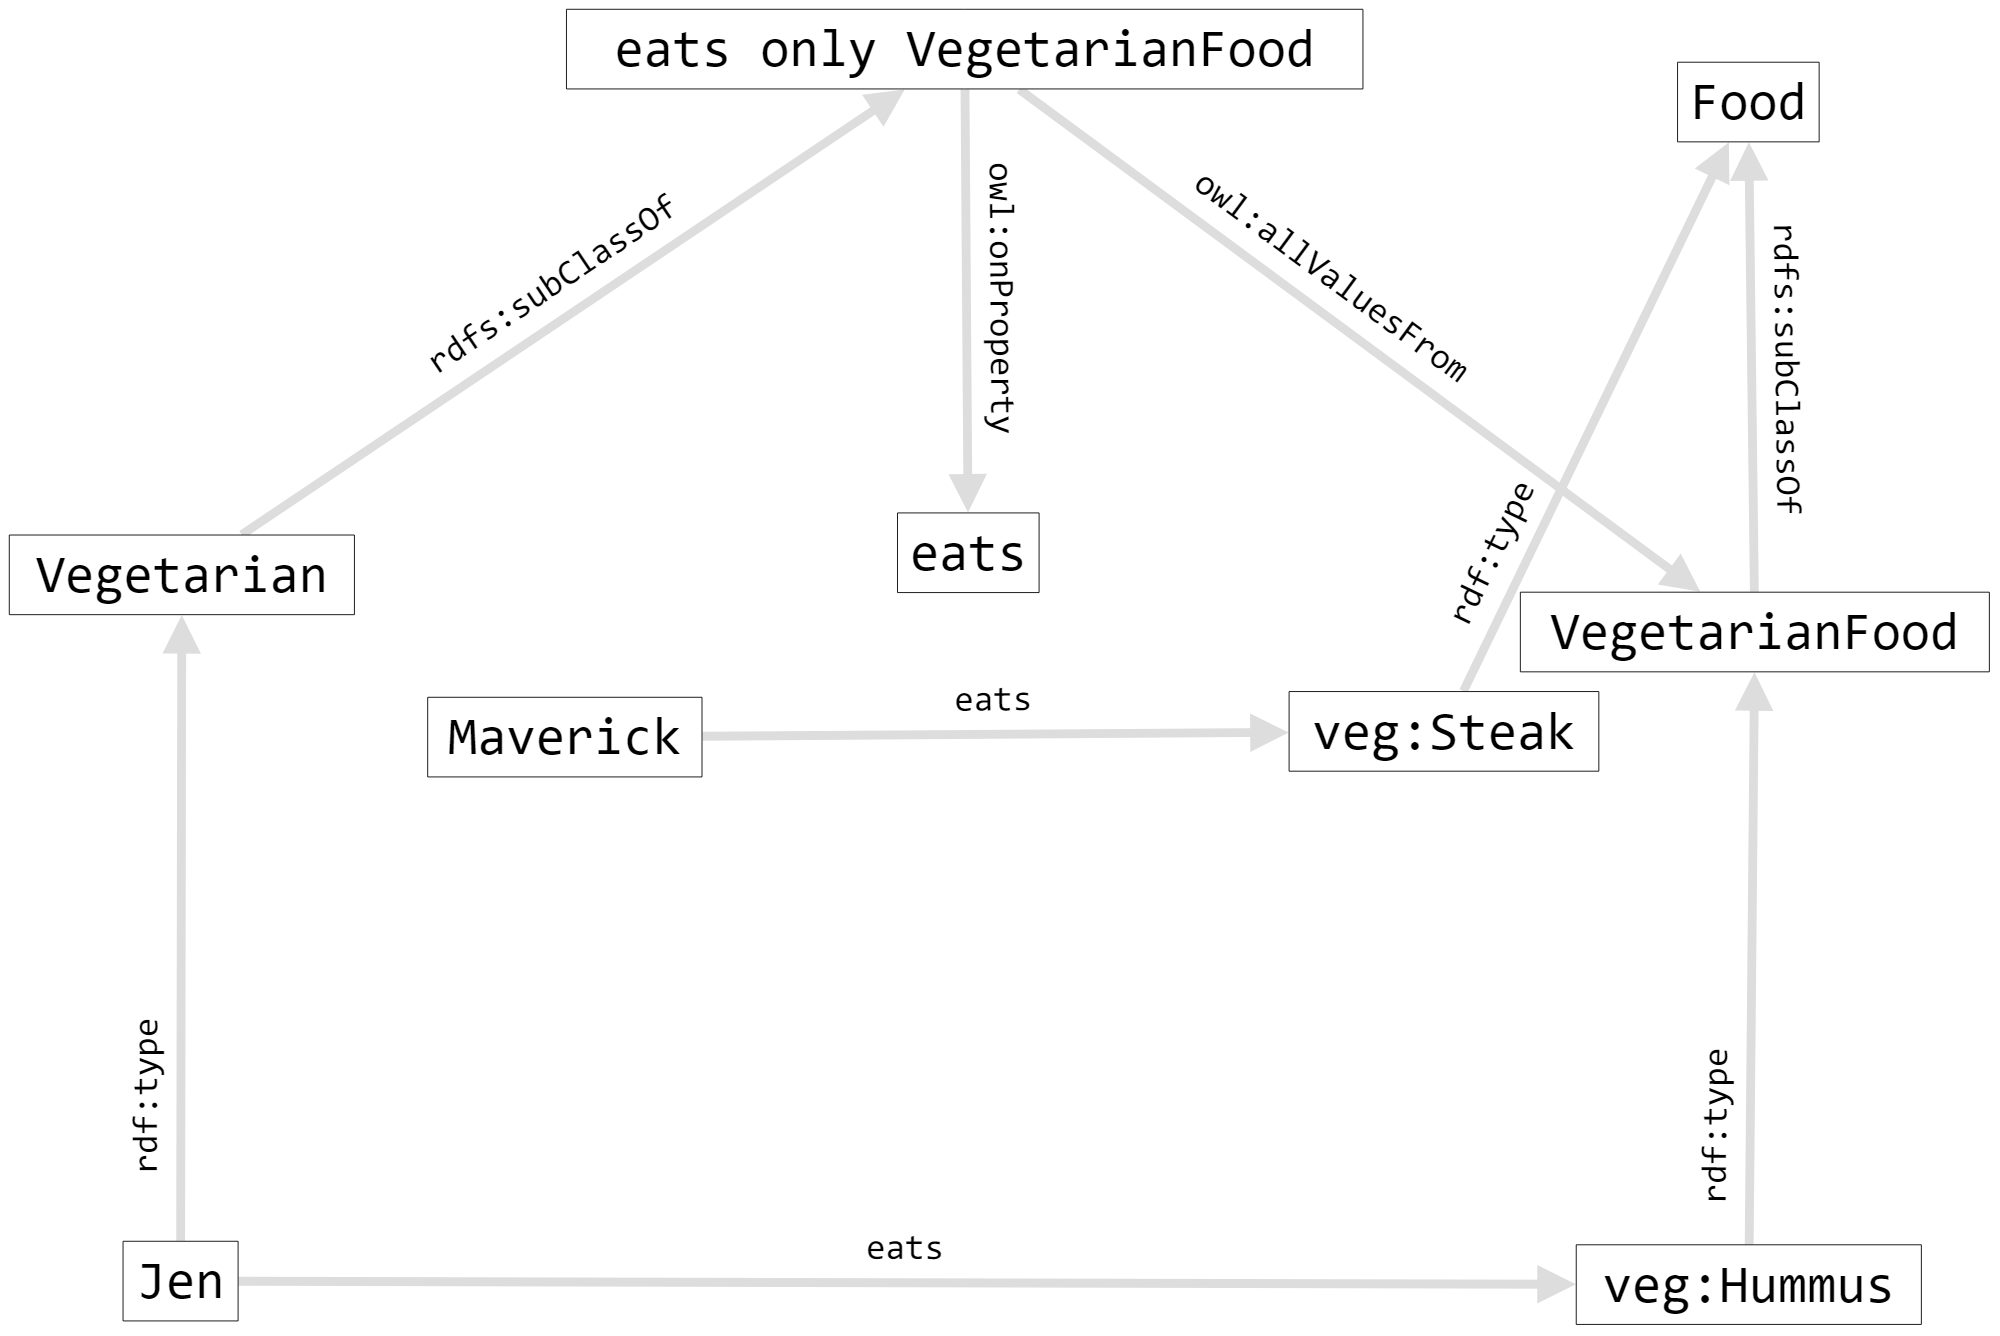
\includegraphics[width=5in]{SWWOv3/media/ch12/figure12-9.png}
\caption{Definition of a vegetarian as a restriction on what the person eats.}
\label{fig:ch12.09}
\end{figure}


\begin{table}[h]
\centering
\begin{tabular}{||l l l l l l l ||} 
 \hline
 ID&Machine Number&Division&ProductLine&Manufacture Location&SKU&Available \\ 
 \hline\hline
1&ZX-3&Manufacturing support&Papermachine&Sacramento&FB3524&23\\
2&ZX-3P&Manufacturing support&Paper machine&Sacramento&KD5243&4\\
3&ZX-3S&Manufacturing support&Paper machine&Sacramento&IL4028&34\\
4&B-1430&Control Engineering&Feedback line&Elizabeth&KS4520&23\\
5&B-1430X&Control Engineering&Feedback line&Elizabeth&CL5934&14\\
6&B-1431&Control Engineering&Active sensor&Seoul&KK3945&0\\
7&DBB-12&Accessories&Monitor&Hong Kong&ND5520&100\\
8&SP-1234&Safety&Safety valve&Cleveland&HI4554&4\\
9&SPX-1234&Safety&Safety valve&Cleveland&OP5333&14\\
\hline
\end{tabular}
\caption{Sample Tabular Data for Triples}
\label{tab:ch12.1}
\end{table}


\begin{table}[h]
\centering
\begin{tabular}{||l l l ||} 
 \hline
 Subject&Predicate&Object \\ 
 \hline\hline
mfg:Product1&mfg:Product\_ID&1 \\
mfg:Product1&mfg:Product\_ModelNo&ZX-3 \\
mfg:Product1&mfg:Product\_Division&Manufacturing support \\
mfg:Product1&mfg:Product\_Product\_Line&Paper machine \\
mfg:Product1&mfg:Product\_Manufacture\_Location&Sacramento \\
mfg:Product1&mfg:Product\_SKU&FB3524 \\
mfg:Product1&mfg:Product\_Available&23 \\
mfg:Product2&mfg:Product\_ID&2\\
mfg:Product2&mfg:Product\_ModelNo&ZX-3P\\
mfg:Product2&mfg:Product\_Division&Manufacturing support \\
mfg:Product2&mfg:Product\_Product\_Line&Paper machine \\
mfg:Product2&mfg:Product\_Manufacture\_Location&Sacramento\\
mfg:Product2&mfg:Product\_SKU&KD5243\\
mfg:Product2&mfg:Product\_Available&4\\
\hline
\end{tabular}
\caption{Triples Representing Some of the Data in Table \protect\ref{tab:ch12.1}}
\label{tab:ch12.2}
\end{table}

\end{challenge}
This is a common situation when actually importing information from a
table. It is quite common for type information to appear as a particular
column in the table. If we use a single method for importing tables, all
the rows become individuals of the same type. A software-intensive
solution would be to write a more elaborate import mechanism that allows
a user to specify which column should specify the type. A model-based
solution would use a model in OWL and an inference engine to solve the
same problem.

\begin{challenge}{Autoclassification in OWL}
\label{ch:Autoclass}

Build a model in OWL so we can infer the type information for each
individual, based on the value in the ``Product\ Line'' 
field but using just the simple imported triples described in
Chapter~\ref{ch3}.

\solution

Since the classes of which the rows will be members (i.e., the product
lines) are already known, we first define those classes:

\begin{lstlisting}
ns:Paper_Machine rdf:type owl:Class .
ns:Feedback_Line rdf:type owl:Class .
ns:Active_Sensor rdf:type owl:Class .
ns:Monitor rdf:type owl:Class .
ns:Safety_Valve rdf:type owl:Class .
\end{lstlisting}

Each of these classes must include just those individuals with the
appropriate value for the property \texttt{mfg:Product\_Product\_Line}. The class
constructor that achieves this uses an owl:hasValue restriction, as
follows:

\begin{lstlisting}
ns:Paper_Machine owl:equivalentClass
    [ a owl:Restriction ;
      owl:onProperty mfg:Product_Product_Line ;
      owl:hasValue "Paper machine" ] .
ns:Feedback_Line owl:equivalentClass
    [ a owl:Restriction ;
      owl:onProperty mfg:Product_Product_Line ;
      owl:hasValue "Feedback line" ] .
ns:Active_Sensor owl:equivalentClass
    [ a owl:Restriction ;
      owl:onProperty mfg:Product_Product_Line ;
      owl:hasValue "Active sensor" ] .
ns:Monitor owl:equivalentClass
    [ a owl:Restriction ;
      owl:onProperty mfg:Product_Product_Line  ;
      owl:hasValue "Monitor" ] .
ns:Safety_Valve owl:equivalentClass
    [ a owl:Restriction ;
      owl:onProperty mfg:Product_Product_Line ;
      owl:hasValue "Safety Valve" ] .
\end{lstlisting}

Each of these definitions draws inferences as desired. Consider
\texttt{mfg:Product1} (``ZX-3''), for which the triple

\begin{lstlisting}
mfg:Product1 mfg:Product_Product_Line "Paper machine".
\end{lstlisting}

has been imported from the table. The first triple ensures that
\texttt{mfg:Product1} satisfies the conditions of the restriction for
Paper\_Machine. Hence,

\begin{lstlisting}
mfg:Product1 rdf:type 
      [ a owl:Restriction; 
        owl:onProperty mfg:Product_Product_Line ;
        owl:hasValue "Paper machine" ].
\end{lstlisting}

can be inferred. Since this restriction is equivalent to the definition
for \texttt{mfg:Paper\_Machine}, we have

\begin{lstlisting}
mfg:Product1 rdf:type mfg:Paper_Machine.
\end{lstlisting}

as desired.

Furthermore, this definition maintains coherence of the data, even if it
came from a source other than the imported table. Suppose that a new
product is defined according to the following RDF:

\begin{lstlisting}
os:ProductA rdf:type mfg:Paper_Machine .
\end{lstlisting}

The semantics of \texttt{owl:equivalentClass} means that all members of
\texttt{mfg:Paper\_ Machine} are also members of the restriction. In particular,

\begin{lstlisting}
os:ProductA rdf:type [ a owl:Restriction;
                       owl:onProperty mfg:Product_Product_Line ;
                       owl:hasValue "Paper Machine" ] .
\end{lstlisting}

Finally, because of the semantics of the restriction, we can infer

\begin{lstlisting}
os:ProductA mfg:Product_Product_Line "Paper Machine".
\end{lstlisting}

The end result of this construct is that regardless of how product
information is brought into the system, it is represented both in terms
of \texttt{rdf:type} and \texttt{mfg:Product\_Product\_Line} consistently.
\end{challenge}

\begin{challenge}{Relating Classes and Individuals}
\label{chal:25}

OWL and RDFS provide considerable modeling power when talking about
classes. In RDFS, we can say that all the members of one class are
members of another. In OWL, we can say things about all the members of a
class---for example, that they all have the value ``Paper\_Machine'' on
the property \texttt{Product\_Product\_Line}. We can use these powerful ways to
relate classes to one another to describe individuals as well. When we
combine these together, we can express rules about how individuals
relate to one another.

We will consider an example from software system management. Suppose we
have a policy that says that all of our desktop applications must
conform to a particular piece of legislation, the Americans with
Disabilities Act of 
1990. How can we express this in RDFS and OWL?

Figure~\ref{fig:ch12.10} shows the model graphically. First we define the set of
desktop applications. A desktop application is something that runs on
the desktop---so we model this with a restriction on the property
runsOn, that it has the value Desktop. This is shown in the top of the
figure. This is a typical pattern for relating a set of things to an
individual; we defined the set of things that run on the desktop to the
individual desktop using a single \texttt{hasValue} restriction.

In the bottom of the figure, we use this pattern again, but this time we
relate the set of applications that comply
with the Americans with Disabilities Act of 1990 (ADA90) with the ADA90
itself, again using a \texttt{hasValue}
restriction.

By building these classes in this way, we can use the modeling power of
OWL and RDFS to express more complex relationships. How do we say that
all the desktop applications must conform to the ADA90? We see this in
the middle of the diagram---we make one restriction a subset of the
other. The figure shows a sample inference--- The desktop supports
MSExcel, which means that MSExcel runs on the desktop (since these two
properties are inverses). This, in turn, means that MSExcel is a desktop
application. But we have asserted that

\begin{lstlisting}
:DesktopApplication rdfs:subClassOf :ConformantApplication .
\end{lstlisting}

This means that MSExcel must also be a conformant application. But
conformant applications conform to the
ADA90; as a member of this class, MSExcel must conform to this as well.
This means that we can infer

\begin{lstlisting}
:MSExcel :conformsTo :ADA90 .
\end{lstlisting}
\end{challenge}

This usage of \texttt{owl:hasValue} is so important that we view it as a design
pattern, and give it a name---the \emph{Class-Individual Mirror} pattern. The
implementation of the pattern is simple---it is a single \texttt{hasValue}
restriction on some property. The interpretation of it is that we are
describing the relationship of an individual to a set---this is the set
of all things that relate to this individual in a certain way. We will
see the importance of this pattern for metamodeling in Section~\ref{metamodel}.

\begin{figure}
\centering
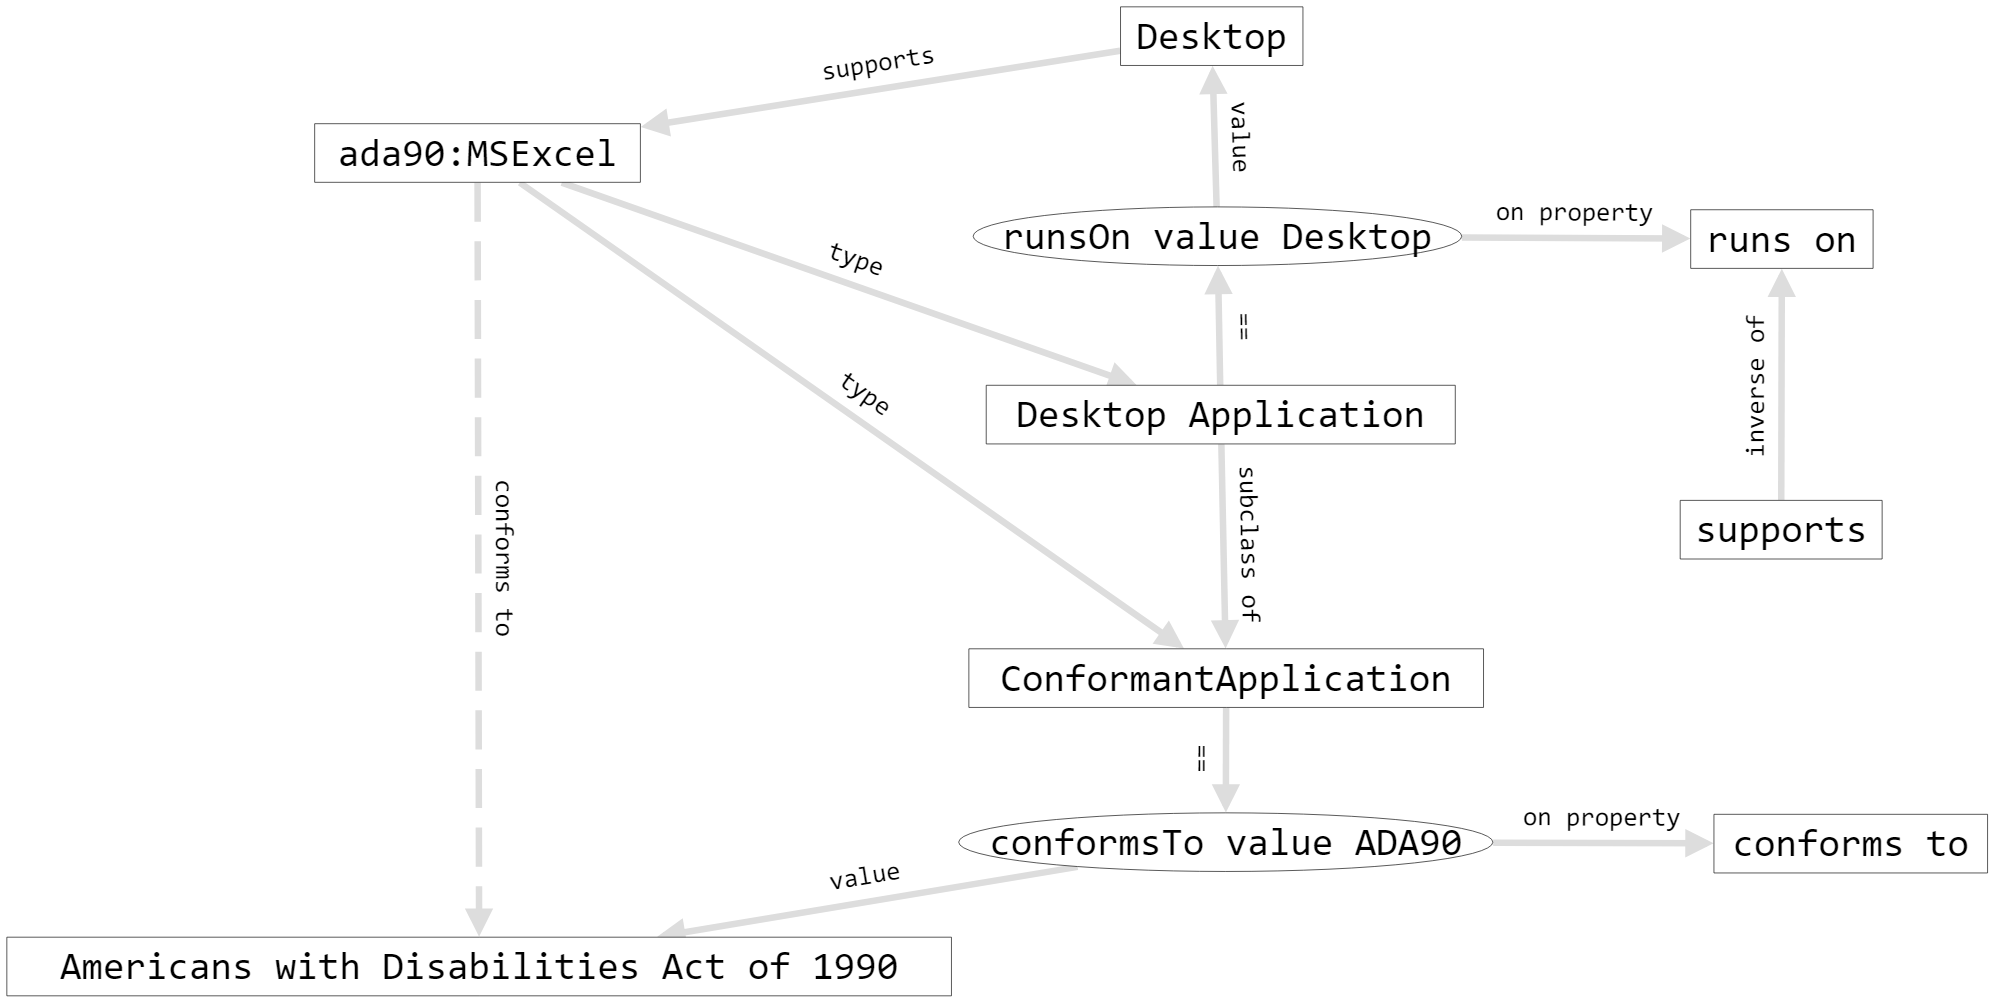
\includegraphics[width=5in]{SWWOv3/media/ch12/figure12-10.png}
\caption{The Americans with Disabilities Act of 1990 as expressed in RDFS and OWL.}
\label{fig:ch12.10}
\end{figure}



\subsection{Relationship transfer}
\label{ch12:Transfer} 

When mapping from one model to another, or even when specifying how one
part of a model relates to another, it is not uncommon to make a
statement of the form ``Everything related to A by property p should
also be related to B but by property q.'' Some examples are ``Everyone
who plays for the All Star team is governed by the league's contract''
and ``Every work in the Collected Works of Shakespeare was written by
Shakespeare.'' We refer to this kind of mapping as relationship
transfer, since it involves transferring individuals in a relationship
with one entity to another relationship with another entity. This
situation arises in FOAF with groups of people. Recall that FOAF
provides two ways to describe members of a group: the \texttt{foaf:member}
relation, which relates an individual member G of \texttt{foaf:Group} to the
individuals who are in that group, and that same group G, which is
related to an \texttt{owl:Class} by the \texttt{foaf:membershipClass} property. We take an
example from the life of Shakespeare to illustrate this.



Suppose we define a \texttt{foaf:Group} for \texttt{Shakespeares\_Children}, as follows:

\begin{lstlisting}
lit:Shakespeares_Children a foaf:Group ;
              foaf:name "Shakespeare's Children" ;
              foaf:member lit:Susanna, lit:Judith, lit:Hamnet ;
	      foaf:membershipClass b:ChildOfShakespeare .
lit:ChildOfShakespeare a owl:Class .
\end{lstlisting}


\begin{figure}
\centering
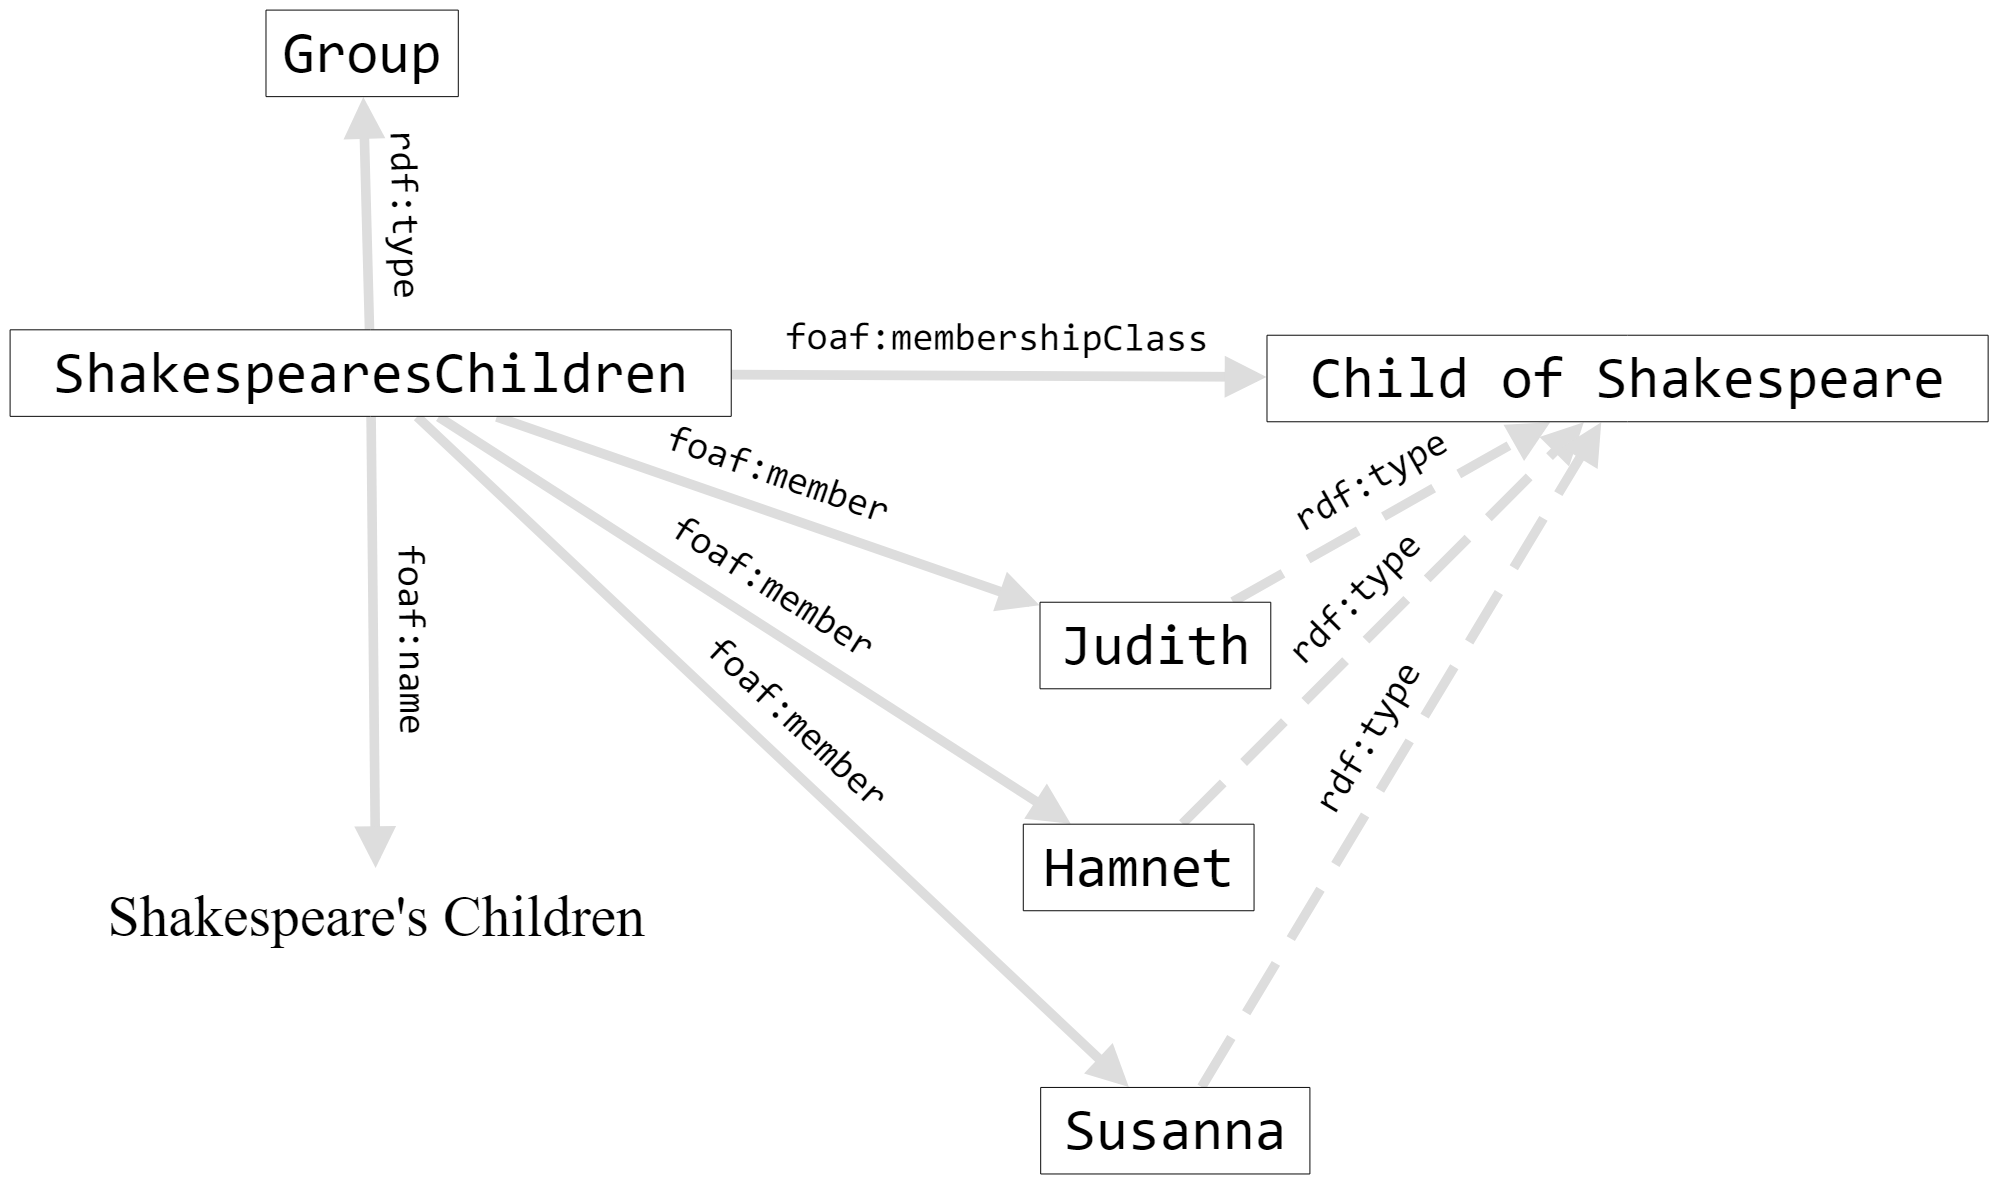
\includegraphics[width=5in]{SWWOv3/media/ch12/figure12-11.png}
\caption{Inferences based on membershipClass in FOAF. FOAF specifies that the
following rule should hold.}
\label{fig:ch12.11}
\end{figure}


FOAF specifies that the following rule should hold: 

\begin{lstlisting}
IF
   lit:Shakespeares_Children foaf:member ?x
THEN
   ?x rdfs:type lit:ChildOfShakespeare
\end{lstlisting}

Figure~\ref{fig:ch12.11} shows graphically the result of this rule in the case of
Shakespeare's family. The fine lines represent asserted triples, and the
three bold lines represent the triples that are to be inferred.


\begin{challenge}{Relationship Transfer in FOAF}
\label{chal:26}

How can we get the inferences shown in Figure\ref{fig:ch12.11} by using only the
constructs from OWL (i.e., without special- purpose rules)?

\solution

For this solution, we are going to define a restriction on a property that points from a member to the \texttt{foaf:Group} it belongs to.  But \texttt{foaf:member} points the wrong way; from the \texttt{Group} to 
the \texttt{member}.  So 
will need to be able to refer to the inverse of \texttt{foaf:mamber}, which we will call \texttt{lit:memberOf}:

\begin{lstlisting}
lit:memberOf owl:inverseOf foaf:member .
\end{lstlisting}

Now we can define \texttt{ChildOfShakespeare} to be (equivalent to) the class of
all individuals who are
\texttt{lit:memberOf} \texttt{lit:Shakespeares\_Children}, using an \texttt{owl:hasValue} restriction:

\begin{lstlisting}
lit:ChildOfShakespeare a owl:Class ;
          rdfs:label "Child of Shakespeare" ;
          owl:equivalentClass
             [ a owl:Restriction ;
               owl:hasValue lit:Shakespeares_Children ;
               owl:onProperty lit:memberOf
             ] .
\end{lstlisting}

Let's follow the progression of Shakespeare's children through this
inference. From Figure~\ref{fig:ch12.11}, we begin with three triples:

\begin{lstlisting}
lit:Shakespeares_Children foaf:member lit:Hamnet.
lit:Shakespeares_Children foaf:member lit:Judith.
lit:Shakespeares_Children foaf:member lit:Susanna.
\end{lstlisting}

By the semantics of \texttt{owl:inverseOf}, we can infer

\begin{lstlisting}
* lit:Hamnet lit:memberOf lit:Shakespeares_Children .
* lit:Judith lit:memberOf lit:Shakespeares_Children .
* lit:Susanna lit:memberOf lit:Shakespeares_Children .
\end{lstlisting}

Therefore, all three are also members of the restriction defined
previously, so we can conclude that

\begin{lstlisting}
* lit:Hamnet rdf:type lit:ChildOfShakespeare.
* lit:Judith rdf:type lit:ChildOfShakespeare.
* lit:Susanna rdf:type lit:ChildOfShakespeare.
\end{lstlisting}

Following similar reasoning, we can also turn this inference around
backward; if we instead assert that

\begin{lstlisting}
lit:Hamnet rdf:type lit:ChildOfShakespeare .
lit:Judith rdf:type lit:ChildOfShakespeare .
lit:Susanna rdf:type lit:ChildOfShakespeare .
\end{lstlisting}

we can infer that

\begin{lstlisting}
* lit:Shakespeares_Children foaf:member lit:Hamnet .
* lit:Shakespeares_Children foaf:member lit:Judith .
* lit:Shakespeares_Children foaf:member lit:Susanna .
\end{lstlisting}

\end{challenge}



We can use the Class-Individual Mirror Pattern in a repeated setting, to 
describe inferences over tree structured data.  Expanding on the pattern 
where we have a class for the children of a famous person, let's go back 
the the example of transitive superproperties from Challenge~\ref{chal:17}.
In that example, we have a family tree of ancestors:

\begin{lstlisting}
:WillemAlexander :haParent :Beatrix.
:Beatrix :hasParent :Wilhelmina .
:hasParent rdfs:subPropertyOf :hasAncestor .
:hasAncestor a owl:TransitiveProperty . 
\end{lstlisting}

Now, let's use the Class Instance Mirror pattern for each of the parents in 
this to describe the descendants of each parent:

\begin{lstlisting}
:DescendantOfWillemAlexander a owl:Class ;
    owl:equivalentClass [ a owl:Restriction ;
                          owl:onProperty anc:hasAncestor ;
                          owl:hasValue :WillemAlexander
                        ] .

:DescendantOfBeatrix a owl:Class ;
     owl:equivalentClass [ a owl:Restriction ;
                           owl:onProperty anc:hasAncestor ;
                           owl:hasValue :Beatrix
                         ] .

:DescendantOfWilhelmina a owl:Class ;
        owl:equivalentClass [ a owl:Restriction ;
                              owl:onProperty :hasAncestor ;
                              owl:hasValue :Wilhelmina
                            ] .
\end{lstlisting}

Now we learn that Willem Alexander has a new addition to his family:

\begin{lstlisting}
:Alexia  a  :DescendentOfWillemAlexander .
\end{lstlisting}

What inferences can we draw?  Evidently, Alexia is a descendant of WillemAlexander
(since she's a member of his descendant class):

\begin{lstlisting}
* anc:Alexia :hasAncestor :WillemAlexander .
\end{lstlisting}

But furthermore, since \texttt{anc:hasAncestor} is a \texttt{owl:TransitiveProperty}, 
we infer

\begin{lstlisting}
* anc:Alexia :hasAncestor :Beatrix, :Wilhelmina .
\end{lstlisting}

But that means that she is a member of their descendant classes as well: 

\begin{lstlisting}
 anc:Alexia a :DescendantOfBeatrix, :DescendantOfWilhelmina .
\end{lstlisting}

But we can generalize this reasoning to hold for any member of WillemAlexanders' descendant class. 
Any such person will have  Willem Alexander as an ancestor, and hence Beatrix and Wilhelmina, 
and therefore a member of \texttt{anc:DescendantOfBeatrix} and 
\texttt{anc:DescendantOfWilhelmina} as well.  This means that we have proven that

\begin{lstlisting}
* anc:DescendantOfWillem rdfs:subClassOf anc:DescendantOfBeatrix .
* anc:DescendantOfBeatrix rdfs:subClassOf anc:DescendantOfWilhelmina .
\end{lstlisting}

This situation is shown in Figure~\ref{fig:ch12.12}.  

\begin{figure}
    \centering
    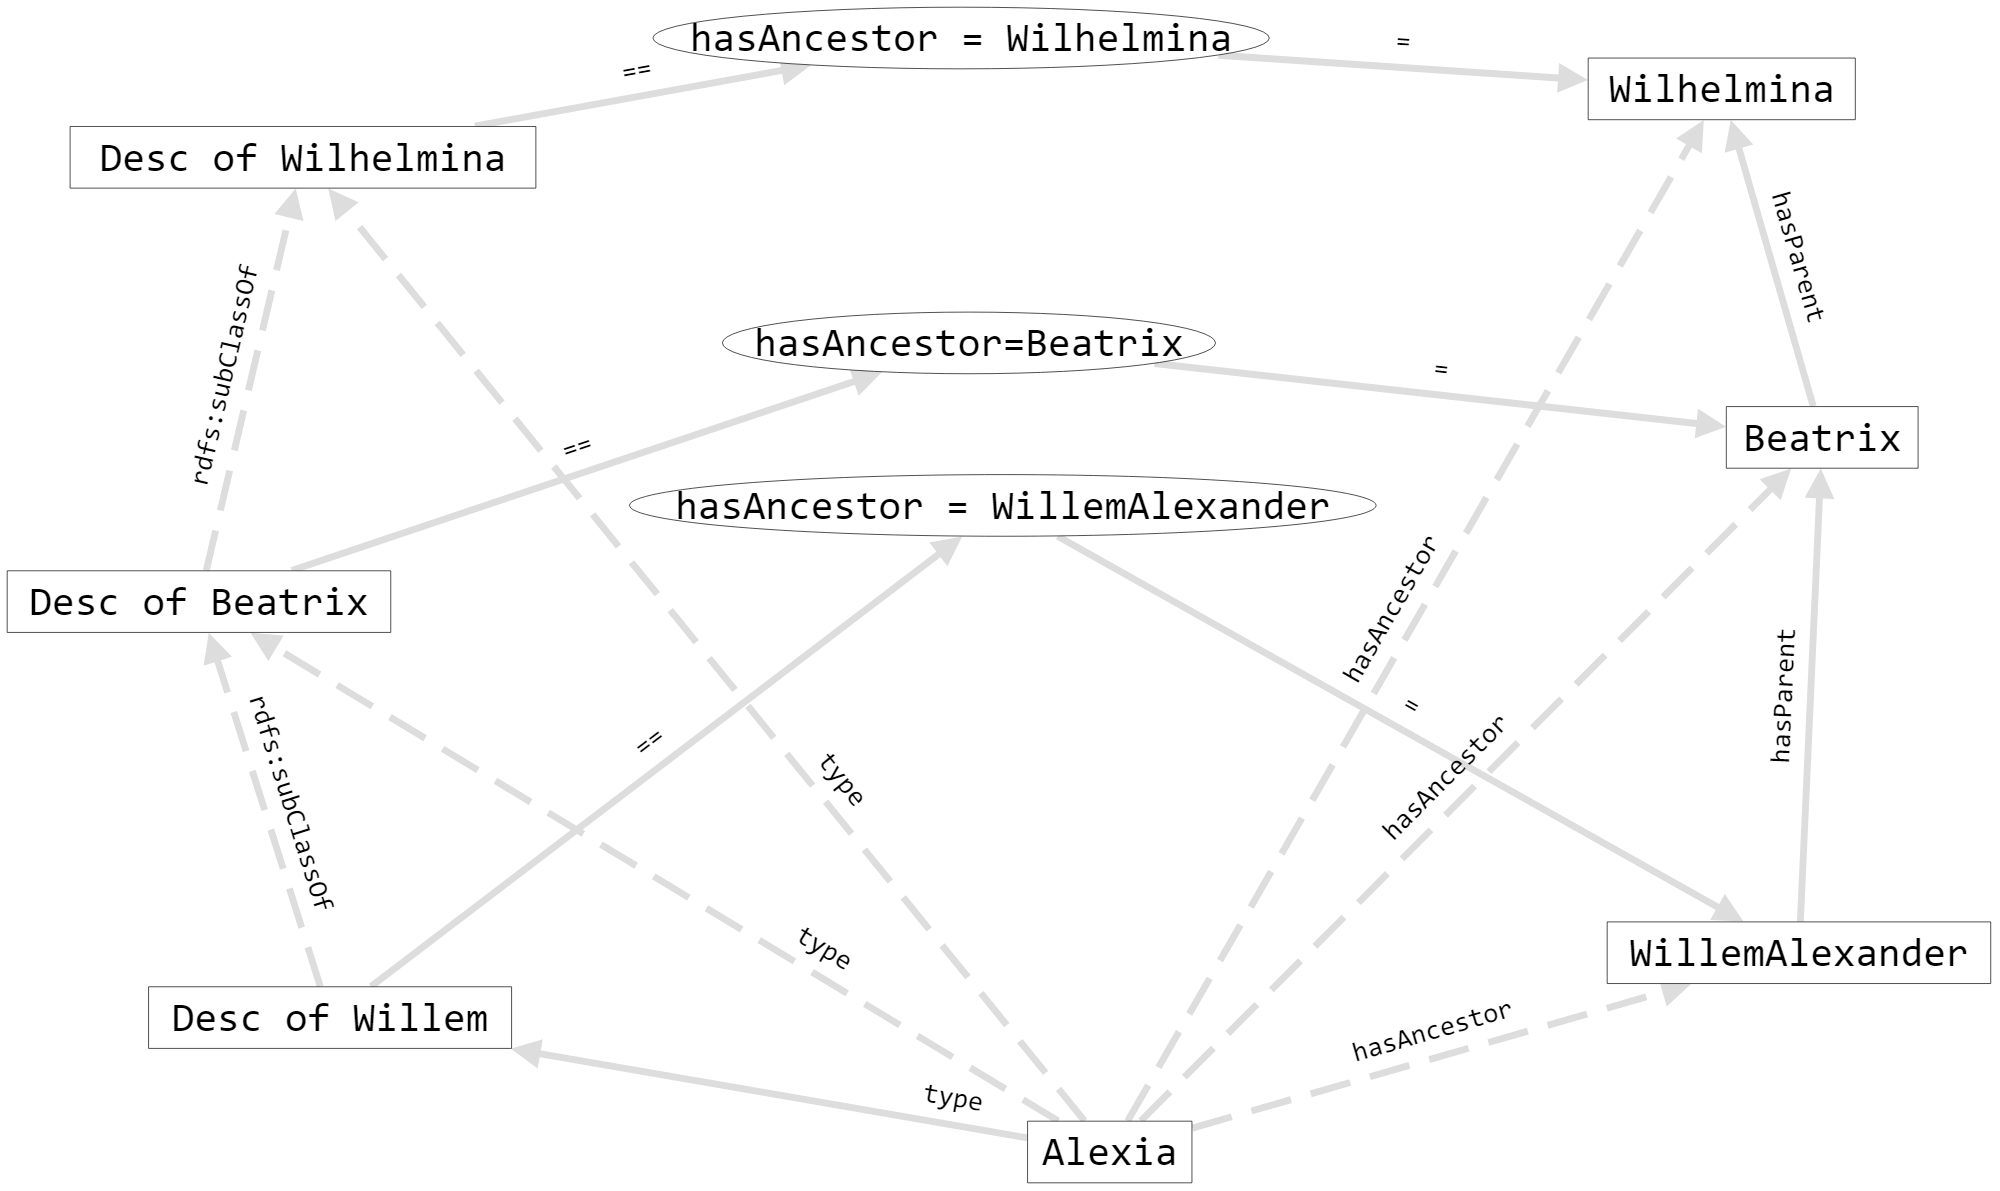
\includegraphics[width=4in]{SWWOv3/media/ch12/figure12-12.png}
    \caption{Inferences from a recursive application of the Class-Individual Mirror pattern}
    \label{fig:ch12.12}
\end{figure}

What are the ramifications of using the Class-Individual Mirror pattern in this way? 
In many modeling situations, there is some controversy about whether something should be 
modeled as a class or as an individual.  Do we want to refer to it as a set of other individuals, 
or do we want to refer to it as a thing in its own right?  Is a species a set of specimens, or
is it a description of its members as a phenotype or genotype?  Is a genre a set of literary 
works, or a topic you can write about?  Is a Dewey Decimal header a set of books, or an entry
in a classification system?  The Class-Individual Mirror pattern shows how both of these 
situations can be modeled, using OWL to specify how they are to be kept in sync.  Additions 
to the individual side (like the addition of Alexia to Willem's family) are reflected on the 
class side.  The whole argument works in reverse; if we assert that Willem's descendants are 
also Beatrix's descendants, then Alexia will have Beatrix as an ancestor as well.  The Class-Individual 
Mirror pattern keeps the two worlds in sync. 

\section{Alternative Descriptions of Restrictions}

In this book, we describe OWL and its semantics with respect to the
interpretation of OWL as RDF triples as defined in the W3C OWL
documents. Other characterizations have been used during the history of
OWL and even appear in user interfaces of some tools. Each
characterization uses its own vocabulary to describe exactly the same
things. In this section we review some of the most common
languages you will encounter when discussing OWL restrictions and
classes, and we also provide a recommendation for best-practice
terminology.

The semantics of rdfs:subClassOf and owl:equivalentClass are quite easy
to characterize in terms of the inferences that hold

\begin{lstlisting}
X rdfs:subClassOf Y.
\end{lstlisting}

can be understood as a simple IF/THEN relation; if something is a member
of X, then it is also a member of Y.

\begin{lstlisting}
X owl:equivalentClass Y.
\end{lstlisting}

can be understood as an IF and only IF relation, that is two IF/THEN
relations, one going each way; if something is a member of X, then it is
also a member of Y, and vice versa.

These relations remain unchanged in the case where X and/or Y are
restrictions. We can see these relationships with examples taken from
the solar system. Consider two classes: one is a named class SolarBody,
which we'll call class A for purposes of this discussion. The other is
the unnamed class defined by a restriction onProperty orbits that it
hasValue TheSun, which we'll call class B. We can say that all solar
bodies orbit the sun by asserting

\begin{lstlisting}
A rdfs:subClassOf B.
\end{lstlisting}

In other words, if something is a solar body, then it orbits the sun.

Other terms are used in the literature for this situation. For example,
it is sometimes described by saying that ``orbiting the sun is a
necessary condition for Solar Body.'' The intuition behind this
description is that if you know that something is a \texttt{SolarBody}, then it
is necessarily the case that it orbits the sun. Since such a description
of the class \texttt{SolarBody} describes the class but does not provide a
complete characterization of it (that is, you cannot determine from this
description that something is a member of \texttt{SolarBody}), then this
situation is also sometimes denoted by saying that ``orbiting the sun is
a partial definition for the class \texttt{SolarBody}.''

If, on the other hand, we say that solar bodies are the same as the set
of things that orbit the sun, we
can express this in OWL compactly as

\begin{lstlisting}
A owl:equivalentClass B.
\end{lstlisting}

Now we can make inferences in both directions: If something orbits the
sun, then it is a \texttt{SolarBody}, and if it is a \texttt{SolarBody}, then it orbits
the sun. This situation is sometimes characterized by saying that
``orbiting the sun is a necessary and sufficient condition for
SolarBody.'' The intuition behind this description is that if you know
something is a \texttt{SolarBody}, then it is necessarily the case that it orbits
the sun. But furthermore, if you want to determine that something is a
\texttt{SolarBody}, it is sufficient to establish that it orbits the sun.
Furthermore, since such a description does fully characterize the class
\texttt{SolarBody}, this situation is also sometimes denoted by saying that
``orbiting the sun is a complete definition for the class SolarBody.''

Finally, if we say that all things that orbit the sun are solar bodies,
we can express this compactly in
OWL as

\begin{lstlisting}
B rdfs:subClassOf A.
\end{lstlisting}

That is, if something orbits the sun, then it is a SolarBody. Given the
usage of the words necessary and sufficient, one could be excused for
believing that in this situation one would say that ``orbiting the sun
is a sufficient condition for SolarBody.'' However, it is not common
practice to use the word sufficient in this way. Despite the obvious
utility of such a statement from a modeling perspective and its
simplicity in terms of OWL (it is no more complex than a partial or
complete definition), there is no term corresponding to partial or
complete for this situation.

Because of the incomplete and inconsistent way the words partial,
complete, sufficient, and necessary have been traditionally used to
describe OWL, we strongly discourage their use and recommend instead the
simpler and consistent use of the OWL terms \texttt{rdfs:subClassOf} and
\texttt{owl:equivalentClass}.

\section{SUMMARY}

A key functionality of OWL is the ability to define restriction classes.
The unnamed classes are defined based on restrictions on the values for
particular properties of the class. Using this mechanism, OWL can be
used to model situations in which the members of a particular class must
have certain properties. In RDFS, the domain and range restrictions can
allow us to make inferences about all the members of a class (such as
playsFor relating a baseball player to a team). In OWL, one can use
restriction statements to differentiate the case between something that
applies to all members of a class versus some members, and even to
insist on a particular value for a specific property of all members of a
class.

When restrictions are used in combination with the constructs of RDFS
(especially rdfs:subPropertyOf and rdfs:subClassOf), and when they are
cascaded with one another (restrictions referring to other
restrictions), they can be used to model complex relationships between
properties, classes, and individuals. The advantage of modeling
relationships in this way (over informal specification) is that
interactions of multiple specifications can be understood and even
processed automatically.

OWL also provides other kinds of restrictions that can be placed on the
members of a class using other kinds of onProperty restrictions. We
discuss these in the next chapter.

\subsection{Fundamental concepts}

The following fundamental concepts were introduced in this chapter.

owl:Restriction---The building block in OWL that describes classes by
restricting the values allowed for certain properties.

owl:hasValue---A type of restriction that refers to a single value for a
property. owl:someValuesFrom---A type of restriction that refers to a
set from which some value for a property must come.

owl:allValuesFrom---A type of restriction that refers to a set from
which all values for a property must come.

owl:onProperty---A link from a restriction to the property it restricts.
